%%%%%%%% ICML 2020 EXAMPLE LATEX SUBMISSION FILE %%%%%%%%%%%%%%%%%

\documentclass{article}

% Recommended, but optional, packages for figures and better typesetting:
\usepackage{microtype}
\usepackage{graphicx}
\usepackage{booktabs} % for professional tables

% For citations
\usepackage{natbib}
\usepackage{amssymb, amsmath,amsthm}
\usepackage{amsfonts}
% For algorithms
\usepackage{algorithm}
\usepackage{algorithmic}
\usepackage{paralist}
\usepackage{multirow}
% Added by Author
% use Times
\usepackage{times}
% For figures
\usepackage{wrapfig}
%\usepackage[authoryear]{natbib}

% For algorithms
\usepackage{url,enumerate}
\usepackage{color,xcolor}
\usepackage{makeidx}  % allows for indexgeneration
\usepackage{amsmath,amssymb}
\usepackage{mathtools}
\usepackage[small, compact]{titlesec}
\usepackage{xspace}
\usepackage{epstopdf}
\usepackage{cite}
% For algorithms
\usepackage{mathrsfs}
\usepackage{times}
\usepackage{enumerate}
\usepackage{color}
\usepackage{graphicx,epsfig}
\usepackage{amsmath,amssymb,xspace}
\usepackage{url}
%\usepackage{subfigure}
\usepackage{hyperref}
\usepackage{bm}
\usepackage{bbm}
\usepackage{upgreek}
\usepackage{cleveref}
\usepackage{multirow}
\usepackage{ulem}
\usepackage{cancel}
%\usepackage{subfig}
\usepackage{subcaption}

% hyperref makes hyperlinks in the resulting PDF.
% If your build breaks (sometimes temporarily if a hyperlink spans a page)
% please comment out the following usepackage line and replace
% \usepackage{icml2018} with \usepackage[nohyperref]{icml2018} above.
\usepackage{hyperref}

% Attempt to make hyperref and algorithmic work together better:
\newcommand{\theHalgorithm}{\arabic{algorithm}}

% Use the following line for the initial blind version submitted for review:
\usepackage{icml2020}

% If accepted, instead use the following line for the camera-ready submission:
%\usepackage[accepted]{icml2018}

% The \icmltitle you define below is probably too long as a header.
% Therefore, a short form for the running title is supplied here:
\icmltitlerunning{Self-Modulating Nonparametric  Event-Tensor Factorization}


\newcommand{\ours}{{{our model}}\xspace}
%\newcommand{\ours}{{\textsc{DiTucker}}\xspace}
\newcommand{\oursw}{\textsc{Ours}\ensuremath{_{\textrm{W}}}\xspace}
\newcommand{\oursu}{\textsc{Ours}\ensuremath{_{\textrm{U}}}\xspace}
\newcommand{\oursg}{\textsc{Ours}\ensuremath{_{\textrm{G}}}\xspace}
%\newcommand{\hadoop}{{Hadoop}\xspace}
\newcommand{\hadoop}{\textsc{Hadoop}\xspace}
\newcommand{\mapreduce}{\textsc{MapReduce}\xspace}
\newcommand{\spark}{\textsc{SPARK}\xspace}
\newcommand{\map}{\textsc{Map}\xspace}
\newcommand{\mapper}{\textsc{Mapper}\xspace}
\newcommand{\mappers}{\textsc{Mappers}\xspace}
\newcommand{\reduce}{\textsc{Reduce}\xspace}
\newcommand{\reducer}{\textsc{Reducer}\xspace}
\newcommand{\InfTuckerEx}{{InfTuckerEx}\xspace}
\newcommand{\InfTucker}{{InfTucker}\xspace}
\newcommand{\tucker}[1]{[\![#1]\!]}
\newcommand{\cbr}[1]{\left\{#1\right\}}
\newcommand{\myspan}[1]{\mathrm{span}\cbr{#1}}
\newcommand{\zsdcaa}[1]{[\textcolor{blue}{zhe's comment: #1}]}
\newcommand{\alanc}[1]{}
\newcommand{\expec}[2]{\EE_{{#1}}\sbr{{#2}}}
\newcommand{\oline}[1]{{\overline{#1}}}
\newcommand{\email}[1]{\href{mailto:#1}{#1}}
\newcommand{\zsdc}[1]{}
\newtheorem{theorem}{Theorem}[section]
\newtheorem{corollary}{Corollary}[theorem]
\newtheorem{lem}[theorem]{Lemma}
\newcommand{\Wei}[1]{{\color{blue}#1}}


% Math commands by Thomas Minka
\newcommand{\var}{{\rm var}}
\newcommand{\Tr}{^{\rm T}}
\newcommand{\vtrans}[2]{{#1}^{(#2)}}
\newcommand{\kron}{\otimes}
\newcommand{\schur}[2]{({#1} | {#2})}
\newcommand{\schurdet}[2]{\left| ({#1} | {#2}) \right|}
\newcommand{\had}{\circ}
\newcommand{\diag}{{\rm diag}}
\newcommand{\invdiag}{\diag^{-1}}
\newcommand{\rank}{{\rm rank}}
% careful: ``null'' is already a latex command
\newcommand{\nullsp}{{\rm null}}
\newcommand{\tr}{{\rm tr}}
\renewcommand{\vec}{{\rm vec}}
\newcommand{\vech}{{\rm vech}}
\renewcommand{\det}[1]{\left| #1 \right|}
\newcommand{\pdet}[1]{\left| #1 \right|_{+}}
\newcommand{\pinv}[1]{#1^{+}}
\newcommand{\erf}{{\rm erf}}
\newcommand{\hypergeom}[2]{{}_{#1}F_{#2}}

% boldface characters
\renewcommand{\a}{{\bf a}}
\renewcommand{\b}{{\bf b}}
\renewcommand{\c}{{\bf c}}
\renewcommand{\d}{{\rm d}}  % for derivatives
\newcommand{\e}{{\bf e}}
\newcommand{\f}{{\bf f}}
\newcommand{\g}{{\bf g}}
\newcommand{\h}{{\bf h}}
%\newcommand{\k}{{\bf k}}
% in Latex2e this must be renewcommand
\renewcommand{\k}{{\bf k}}
\newcommand{\m}{{\bf m}}
\newcommand{\mb}{{\bf m}}
\newcommand{\n}{{\bf n}}
\renewcommand{\o}{{\bf o}}
\newcommand{\p}{{\bf p}}
\newcommand{\q}{{\bf q}}
\renewcommand{\r}{{\bf r}}
\newcommand{\s}{{\bf s}}
\renewcommand{\t}{{\bf t}}
\renewcommand{\u}{{\bf u}}
\renewcommand{\v}{{\bf v}}
\newcommand{\w}{{\bf w}}
\newcommand{\x}{{\bf x}}
\newcommand{\y}{{\bf y}}
\newcommand{\z}{{\bf z}}
%s\newcommand{\l}{\boldsymbol{l}}
\newcommand{\A}{{\bf A}}
\newcommand{\B}{{\bf B}}
\newcommand{\C}{{\bf C}}
\newcommand{\D}{{\bf D}}
\newcommand{\E}{{\bf E}}
\newcommand{\F}{{\bf F}}
\newcommand{\G}{{\bf G}}
\renewcommand{\H}{{\bf H}}
\newcommand{\I}{{\bf I}}
\newcommand{\J}{{\bf J}}
\newcommand{\K}{{\bf K}}
\renewcommand{\L}{{\bf L}}
\newcommand{\M}{{\bf M}}
%\newcommand{\Mcal}{{\mathcal{M}}}
\newcommand{\N}{\mathcal{N}}  % for normal density
\newcommand{\MN}{\mathcal{MN}} 
\newcommand{\Acal}{\mathcal{A}}
\newcommand{\Bcal}{\mathcal{B}}
\newcommand{\Ccal}{\mathcal{C}}
\newcommand{\Dcal}{\mathcal{D}}
\newcommand{\Ocal}{\mathcal{O}}
\newcommand{\Ycal}{\mathcal{Y}}
\newcommand{\Zcal}{\mathcal{Z}}
\newcommand{\Fcal}{\mathcal{F}}
\newcommand{\Vcal}{\mathcal{V}}
\newcommand{\Lcal}{\mathcal{L}}
\newcommand{\Tcal}{\mathcal{T}}
\newcommand{\Gcal}{\mathcal{G}}
\newcommand{\Hcal}{\mathcal{H}}
\newcommand{\Scal}{\mathcal{S}}

%\newcommand{\N}{{\bf N}}
\renewcommand{\O}{{\bf O}}
\renewcommand{\P}{{\bf P}}
\newcommand{\Q}{{\bf Q}}
\newcommand{\R}{{\bf R}}
\renewcommand{\S}{{\bf S}}
\newcommand{\T}{{\bf T}}
\newcommand{\U}{{\bf U}}
\newcommand{\V}{{\bf V}}
\newcommand{\W}{{\bf W}}
\newcommand{\X}{{\bf X}}
\newcommand{\Y}{{\bf Y}}
\newcommand{\Z}{{\bf Z}}
\newcommand{\Mcal}{{\mathcal{M}}}
\newcommand{\Wcal}{{\mathcal{W}}}
\newcommand{\Ucal}{{\mathcal{U}}}


% this is for latex 2.09
% unfortunately, the result is slanted - use Latex2e instead
%\newcommand{\bfLambda}{\mbox{\boldmath$\Lambda$}}
% this is for Latex2e
\newcommand{\bfLambda}{\boldsymbol{\Lambda}}

% Yuan Qi's boldsymbol
\newcommand{\bsigma}{\boldsymbol{\sigma}}
\newcommand{\balpha}{\boldsymbol{\alpha}}
\newcommand{\bpsi}{\boldsymbol{\psi}}
\newcommand{\bphi}{\boldsymbol{\phi}}
\newcommand{\boldeta}{\boldsymbol{\eta}}
\newcommand{\Beta}{\boldsymbol{\eta}}
\newcommand{\btau}{\boldsymbol{\tau}}
\newcommand{\bvarphi}{\boldsymbol{\varphi}}
\newcommand{\bzeta}{\boldsymbol{\zeta}}
\newcommand{\bepi}{{\boldsymbol{\epsilon}}}

\newcommand{\blambda}{\boldsymbol{\lambda}}
\newcommand{\bLambda}{\mathbf{\Lambda}}
\newcommand{\bOmega}{\mathbf{\Omega}}
\newcommand{\bomega}{\mathbf{\omega}}
\newcommand{\bPi}{\mathbf{\Pi}}

\newcommand{\btheta}{\boldsymbol{\theta}}
\newcommand{\bpi}{\boldsymbol{\pi}}
\newcommand{\bxi}{\boldsymbol{\xi}}
\newcommand{\bSigma}{\boldsymbol{\Sigma}}

\newcommand{\bgamma}{\boldsymbol{\gamma}}
\newcommand{\bGamma}{\mathbf{\Gamma}}

\newcommand{\bmu}{\boldsymbol{\mu}}
\newcommand{\1}{{\bf 1}}
\newcommand{\0}{{\bf 0}}

% \newcommand{\comment}[1]{}

\newcommand{\bs}{\backslash}
\newcommand{\ben}{\begin{enumerate}}
\newcommand{\een}{\end{enumerate}}

 \newcommand{\notS}{{\backslash S}}
 \newcommand{\nots}{{\backslash s}}
 \newcommand{\noti}{{\backslash i}}
 \newcommand{\notj}{{\backslash j}}
 \newcommand{\nott}{\backslash t}
 \newcommand{\notone}{{\backslash 1}}
 \newcommand{\nottp}{\backslash t+1}
% \newcommand{\notz}{\backslash z}

\newcommand{\notk}{{^{\backslash k}}}
%\newcommand{\noti}{{^{\backslash i}}}
\newcommand{\notij}{{^{\backslash i,j}}}
\newcommand{\notg}{{^{\backslash g}}}
\newcommand{\wnoti}{{_{\w}^{\backslash i}}}
\newcommand{\wnotg}{{_{\w}^{\backslash g}}}
\newcommand{\vnotij}{{_{\v}^{\backslash i,j}}}
\newcommand{\vnotg}{{_{\v}^{\backslash g}}}
\newcommand{\half}{\frac{1}{2}}
\newcommand{\msgb}{m_{t \leftarrow t+1}}
\newcommand{\msgf}{m_{t \rightarrow t+1}}
\newcommand{\msgfp}{m_{t-1 \rightarrow t}}

\newcommand{\proj}[1]{{\rm proj}\negmedspace\left[#1\right]}
\newcommand{\argmin}{\operatornamewithlimits{argmin}}
\newcommand{\argmax}{\operatornamewithlimits{argmax}}

\newcommand{\dif}{\mathrm{d}}
\newcommand{\abs}[1]{\lvert#1\rvert}
\newcommand{\norm}[1]{\lVert#1\rVert}

%miscellaneous symbols
%\newcommand{\ie}{{{\em i.e.,}}\xspace}
\newcommand{\ie}{{\textit{i.e.,}}\xspace}
\newcommand{\eg}{{\textit{e.g.,}}\xspace}
\newcommand{\etc}{{\textit{etc.}}\xspace}
\newcommand{\EE}{\mathbb{E}}
\newcommand{\expt}[2]{\EE_{#1}\big[#2\big]}
\newcommand{\dr}[1]{\nabla #1}
\newcommand{\VV}{\mathbb{V}}
\newcommand{\sbr}[1]{\left[#1\right]}
\newcommand{\rbr}[1]{\left(#1\right)}
\newcommand{\cmt}[1]{}


\newcommand{\bi}{{\bf i}}
\newcommand{\bj}{{\bf j}}
\newcommand{\bK}{{\bf K}}
\newcommand{\Vtr}{\mathrm{Vec}}
\newcommand{\tlam}{{\tilde{\lambda}}}
\newcommand{\kl}{{\mathrm{KL} }}




\begin{document}

\twocolumn[
\icmltitle{Self-Modulating Nonparametric Event-Tensor Factorization}


\vskip 0.3in
]


%tensor decomposition framework, don't let other feel incremental 
\begin{abstract}
Tensor factorization is a fundamental framework to analyze high-order interactions in data. Despite the success of the existing methods, the valuable temporal information are severely underused. The timestamps of the interactions are either ignored or discretized into crude steps. The recent work although formulates event-tensors to keep the timestamps in factorization and can capture mutual excitation effects among the interaction events, it overlooks another important type of temporal influence, \textit{inhibition}. In addition, it uses a local window to exclude all the long-term dependencies. To overcome these limitations, we propose a self-modulating nonparametric Bayesian factorization model. We use the latent factors to construct mutually-governed, general random point processes, which can capture various short-term/long-term, excitation/inhibition effects, so as to encode the complex temporal dependencies into factor representations.  In addition, our model couples with a latent Gaussian process to estimate and fuse nonlinear yet static relationships between the entities. For efficient inference, we derive a fully decomposed model evidence lower bound to dispense with the huge kernel matrix and costly summations inside the rate and log rate functions. We then develop an efficient stochastic optimization algorithm. We show the advantage of our method in four real-world applications. 
\end{abstract}		

\section{Introduction}
Interactions between multiple entities (or nodes) are common in real-world applications. For example, consumers' activities can be viewed as interactions between \textit{customers}, \textit{service items} and \textit{providers}. These (high-order) interactions are naturally represented by tensors and analyzed by tensor factorization, which learns a set of latent factors to represent each participant. With the factor representations, we can discover the hidden structures within the entities, \eg clusters and outliers, and extract useful features to make predictions (in downstream tasks). 

While many excellent methods for tensor factorization have been proposed~\citep{Tucker66,Harshman70parafac,Chu09ptucker,kang2012gigatensor,choi2014dfacto}, they mainly conduct a multilinear decomposition, and might  be inadequate to capture more complex, nonlinear relationships. More importantly, they severely underuse the valuable temporal information along with the data. Most methods either drop the time stamps of the interactions,  summarizing the events as a count tensor~\citep{chi2012tensors, HaPlKo15, Hu2015CountTensor}, or discretize the time stamps into crude steps (\eg weeks or months), ignoring the temporal dependencies  in the same step~\citep{xiong2010temporal, schein2015bayesian, Schein:2016:BPT:3045390.3045686}.  Recently, \citet{zhe2018stochastic} formulates event-tensors (where the tensor entries are sequences of interaction events) to preserve the accurate timestamps. They used Hawkes processes to estimate the fine-grained, triggering effects between the interactions. However, their approach overlooks \textit{inhibition}, another ubiquitous effect between the events, and can still miss important temporal patterns. In addition, to compromise on the computational cost, they use a small time window to restrict the range of dependent events, and cannot capture long-term temporal influences of the interactions. 

%our approach
To overcome these limitations, we propose a self-modulating nonparametric Bayesian factorization model for event tensors, which not only can capture static, nonlinear  relationships of the entities, but also is flexible enough to capture a variety of short-term and long-term, excitation and inhibition effects among the interaction events, encoding these complex temporal effects into the factor representations.  Specifically, we use the latent factors to construct a set of mutually-governed, general random point processes to sample the observed interaction events. We first use a latent Gaussian process (GP) to sample a function of the factor representations to determine the type of temporal effect between each pair of interactions. The strength of the effect is further modelled as a kernel (similarity) function of their factors. In this way, both the type  and strength of the effect are absorbed into the factors, from which we can discover the underlying temporal structures. We then couple with another latent GP to sample the base rate as a (nonlinear) function of the factors, in order to estimate and fuse complex yet  static relationships between the entities. We use a scaled softplus function to additively integrate all the positive and negative influences from previous interactions to construct the rate function. For efficient inference, we take advantage of the convexity and log concavity of the rate function, and use the sparse variational GP framework~\cite{hensman2013gaussian} and Jensen's inequality to derive a fully decomposed model evidence lower bound (ELBO). Based on the ELBO, we develop an efficient stochastic optimization algorithm. The complexity of our algorithm is only proportional to the size of the mini-batches, while it captures all the long-term dependencies among the interactions. 


%evaluation
For evaluation, we examined our method on four real-world datasets. Our model nearly always achieves better predictive performance than the existing methods using Poisson processes, time factors, and Hawkes processes to incorporate temporal information. The training curves show that our inference algorithm converges reasonably fast and is resistant to overfitting. Finally, by looking into the latent factors estimated by our approach, we found interesting/meaningful structures both within the entities and within the events. We also found interesting temporal influence patterns.   


%\vspace{-0.1in}
\section{Background}
%\vspace{-0.1in}
\textbf{Tensor Factorization.} We denote a $K$-mode tensor by $\Ycal \in \mathbb{R}^{d_1 \times \ldots \times d_K}$. The $k$-th mode includes $d_k$ entities or nodes (\eg customers).  Each entry is indexed by a tuple $\bi = (i_1, \ldots, i_K)$ and stands for the interaction of the corresponding $K$ nodes.  The entry value is denoted by $y_{\bi}$. To decompose $\Ycal$, we  introduce $K$ latent factor matrices $\Ucal = \{\U^1, \ldots, \U^K\}$ to represent all the tensor nodes. Each $\U^k =[\u^k_1; \ldots ; \u^k_{d_k}]^\top$, which is $d_k \times r_k$, and each $\u^k_t$ are the $r_k$ latent factors of node $t$ in mode $k$. We aim to use $\Ucal$ to recover the observed entries in $\Ycal$. A classical approach is Tucker decomposition~\citep{Tucker66}, which assumes $\Ycal = \Wcal \times_1 \U^{1} \times_2 \ldots \times_K \U^{K}$, where  $\mathcal{W} \in \mathbb{R}^{r_1 \times \ldots \times r_K}$ is a parametric tenor,  and $\times_k$ is the mode-$k$ tensor matrix product~\citep{kolda2006multilinear}, which resembles the ordinary matrix-matrix product.
If we set all $r_k = r$ and $\Wcal$ to be diagonal, Tucker decomposition becomes  CANDECOMP/PARAFAC (CP) decomposition~\citep{Harshman70parafac}. While numerous tensor factorization methods have  been proposed, \eg  ~\citep{Chu09ptucker,kang2012gigatensor,choi2014dfacto}, most of them are inherently based on the CP or Tucker form. However, since both forms are mutilinear to the latent factors, they are incapable of capturing more complicated, nonlinear relationships in data.

\textbf{Factorization with Temporal Information.} Real-world tensors are often supplemented with detailed temporal information, namely, the timestamps of the observed interactions.

To incorporate these information, traditional methods either  drop the timestamps  to perform count tensor decomposition~\citep{chi2012tensors, Hu2015CountTensor}, or  discretize the timestamps into time steps, \eg weeks or months,  augment the tensor with a time mode~\citep{xiong2010temporal, schein2015bayesian, Schein:2016:BPT:3045390.3045686}, and jointly estimate the time factors. Both approaches can be viewed as using Poisson processes to model the interaction events, $p(y_\bi) \propto e^{-\lambda_{\bi}T}\lambda_{\bi}^{y_\bi}$,  where $y_\bi$ is the interaction count in entry $\bi$ (with/without a time step), and $\lambda_{\bi}$ is the event rate.  The factorization is performed on $\{\lambda_{\bi}\}$ or $\{\log(\lambda_{\bi})\}$, typically with Tucker/CP forms. 
Despite their simplicity and convenience, these methods disregard the rich and vital temporal dependencies between the interactions, due to the independent increment assumption in Poisson processes.  To mitigate this issue, \citet{zhe2018stochastic} formulated \textit{event-tensor} to maintain all the accurate timestamps. In an event-tensor, each entry is an event sequence of a particular interaction, rather than a numerical value. \citet{zhe2018stochastic} modelled the observed entries as a set of mutually excited Hawkes processes~\citep{hawkes1971spectra}. The rate of the events in each entry  $\bi$ is
\begin{align}
\lambda_\bi(t) = \lambda_\bi^0 + \sum\nolimits_{s_n \in A(t)} k(\x_{\bi_n},\x_{\bi})h_0(t-s_n) \label{eq:rate-1}
\end{align}
where $\lambda_\bi^0$ is the background rate, $A(t)$ is a local time window that specifies the range of dependent events happened before $t$ (\eg  $50$ past events nearest to $t$), $\bi_n$ is the entry which the previous interaction at time $s_n$ belongs to, $\x_{\bi_n}$ and $\x_{\bi}$ are the latent factors associated with entry $\bi_n$ and $\bi$ respectively, $k(\cdot, \cdot)$ is a kernel function that measures their similarity, and $h_0(\cdot)$ is a base triggering kernel that measures how the triggering effect decays along with time. From the rate function \eqref{eq:rate-1}, we can see that the model can capture the (local) excitation effects of the previously happened interactions on the current one, and the triggering strength are (partly) encoded into the latent factors --- the closer the corresponding factors of the two entries, the stronger the strength. 

\section{Model}
%\vspace{-0.05in}
Although \citet{zhe2018stochastic}'s model can capture fine-grained, mutual triggering effects among the interactions, it ignores another important class of temporal influence --- \textit{inhibition}. The inhibition effect between the events are ubiquitous in real world. For example, a customer who has recently purchased a Surface laptop is unlikely to buy an MacBook; people who voted for one president candidate are unlikely to support another candidate in a short term. In practice, among the interaction events can be mixed excitation and inhibition effects, resulting in complex temporal dependencies. In addition, the model uses a local time window $A(t)$ to specify a small range of the dependent events for each interaction (see \eqref{eq:rate-1}). Although this can save much computational cost for the rate function and its logarithm in model estimation (especially for a large number of events),  it excludes all the long-term  influences of the interaction events on each other, and hence can miss many interesting and valuable temporal patterns. To overcome these problems, we propose a self-modulating nonparametric Bayesian event-tensor factorization model, presented as follows.

\subsection{Notations for Event-Tensor}

First, let us supplement a few notations. In the event-tensor, for each observed entry $\bi$, we denote its event sequence by $y_{\bi} = [s_\bi^1, \ldots, s_\bi^{n_\bi}]$, \ie the time stamps the interaction $\bi$ occurred, and $n_\bi$ is the number of occurrences. Note that each entry represents a particular type of interaction. We can merge the event sequences of all the observed entries into a single sequence, $S = [(s_1, \bi_1). \ldots, (s_N, \bi_N)]$, where $s_1 \le \ldots \le s_N$ are all the time stamps, each $\bi_n$  indexes the entry that event $s_n$ belongs to, \ie the particular interaction occurred at $s_n$. 
%\vspace{-0.1in}
\subsection{Self-Modulating Nonparametric Factorization}
%\vspace{-0.05in}
%the motivation to introduce the g func. 
We now consider to use the latent factors $\Ucal$ to construct a general random point process to accommodate  both the triggering and inhibition effects among the interaction events. One basic assumption in \citep{zhe2018stochastic}  (see \eqref{eq:rate-1}) is that the closer (or more similar) the factor representations of two interactions, the stronger their mutual excitation effects. This is true in many applications, for example, ``the event that \textit{user} A purchased \textit{commodity} B may excite A's friend C to purchase B as well''. Obviously, the factors of A and C are expected to be close because they are in the same community (\ie friends) and so are the factor representations for the interactions (A, B) and (C, B).  However, in many other cases,  closer factor representations may on the contrary lead to stronger inhibition effects. For example, the event that user A has purchased Surface laptop B can strongly suppress A to buy MacBook C (aforementioned); the event that athlete A has won the champion of Game B deprives of the possibility that his competitor C wins B. Therefore, to model the strength of the temporal influence of a previously occurred interaction $\bj$ on the current one $\bi$, we still use a kernel function of their factor representations, $k(\x_{\bj}, \x_{\bi})$, where
$\x_{\bi} = [\u^1_{i_1}; \ldots; \u^K_{i_K}]$ and $\x_{\bj} = [\u^1_{j_1}; \ldots; \u^K_{j_K}]$. However, to detect the type of the influence, we consider to learn a discriminative function of the factor representations, $g(\x_{\bj}, \x_{\bi})$, where $g(\x_{\bj}, \x_{\bi})>0$ indicate that $\bj$ will trigger the occurrence of $\bi$ and otherwise inhibit. To flexibly estimate $g(\cdot)$, we place a Gaussian process (GP) prior~\citep{Rasmussen06GP} --- a nonparametric function prior that accommodates various complex functions. Hence, the latent function values $\g$ for every pair of observed entries will follow a multivariate Gaussian distribution, 
\begin{align}
p(\g|\Ucal) = \N\big(\g|\0, \kappa_g(\X_g, \X_g)\big), \label{eq:gp-g}
\end{align}
where each row of the input matrix $\X_g$ corresponds to a pair of entries, and are the concatenation of the associated factors, $\kappa_g(\cdot, \cdot)$ is the covariance (kennel) function. 

Now, we define a raw rate function for each entry $\bi$ that integrates both the triggering and suppressing effects from the previous interactions, 
\begin{align}
&\tlam_{\bi}(t) = \lambda_\bi^0 \notag \\
&+\sum_{s_n<t} \mathrm{tanh}\big(g(\x_{\bi_n} ,\x_\bi)\big)k(\x_{\bi_n} , \x_{\bi})h_0(t-s_n)   \label{eq:raw-rate}
\end{align}
where $\lambda_\bi^0$ is the background rate and $h_0(\cdot)$ is a base kernel that describes the how the strength of the influence decays with time. In our experiments, we chose the commonly used exponential decay kernel, $h_0(\Delta)=\exp(-\frac{\Delta}{\tau})$. Note that we use $\mathrm{tanh}(\cdot)$ to squeeze the values of $g(\cdot)$ into $[-1, 1]$ without changing the sign. The reason is that we use $g(\cdot)$ to just determine the influence types (excitation or inhibition); for clear interpretability, we do not want to confound it with the influence strength (which are modelled by the other components, \ie $k(\cdot, \cdot)$ and $h_0(\cdot)$). 

Next, to obtain a positive rate function so as to build a valid point process, we use a scaled soft-plus function $\gamma_s(\cdot)$ to transform the raw rate $\tlam_{\bi}(t)$, 
\begin{align}
\lambda_{\bi}(t) =\gamma_s\big(\tlam_{\bi}(t)\big) = s \log\big(1 + \exp(\frac{\tlam_{\bi}(t)}{s})\big) \label{eq:rate}
\end{align}
where $s>0$. It is trivial to show that when $s \rightarrow \infty$,  $\lambda_\bi(t)  \rightarrow \max\big(\tlam_\bi(t), 0\big)$. Therefore, the scaled soft-plus can considerably maintain the additive structure in our raw rate definition in \eqref{eq:raw-rate}. While other transformation operators are also possible, \eg $\exp(\cdot)$, we found empirically that the scaled softplus exhibits superior and excellent performance.

Finally, to estimate the complex yet static relationships between the entities and fuse the relationships into the latent factors, we model the background rate $\lambda_\bi^0$ in each entry $\bi$ as a nonlinear function of the associated factors, $f(\x_{\bi})$. To this end, we place another GP prior over $f(\cdot)$. Then the background rate values $\f$ for all the observed entries are sampled from a multivariate Gaussian distribution,
\begin{align}
p(\f|\Ucal) = \N\big(\f|\0, \kappa_f(\X_f, \X_f)\big), \label{eq:gp-f}
\end{align} 
where each row of $\X_f$ are the concatenated factors associated with one entry, and $\kappa_f(\cdot,\cdot)$ is the covariance (or kernel) function. Note that we do not need to constrain $f(\cdot)>0$, because via the soft-plus transformation \eqref{eq:rate}, we will always obtain a non-negative event rate. 

We place a standard Gaussian prior over all the latent factors $\Ucal$. Given the observed interaction events $\Scal$ (from all the entries), the joint probability of our model is given by 
\begin{align}
&p(\Scal, \g, \f, \Ucal) = \prod_k\prod_{i_k} \N(\u_{i_k}^k|\0, \I) \notag \\
&\cdot \N\big(\g|\0, \kappa_g(\X_g, \X_g)\big) \N\big(\f|\0, \kappa_f(\X_f, \X_f)\big) \notag \\
&\cdot \prod_{\bi} \exp\big(-\int_0^T \lambda_{\bi}(t)\d t\big) \prod_{n=1}^N \lambda_{\bi_n}(s_n) \label{eq:joint}
\end{align}
where $T$ is the total time span across all the events. Note that the last row is the likelihood of our proposed mutually governed, general random point process on the observed entries~\citep{daley2007introduction}.
\vspace{-0.1in}
\section{Algorithm}
\vspace{-0.05in}
The estimation of our model is challenging. First, the exact inference of our model is infeasible for large data because the GP likelihoods \eqref{eq:gp-g} and \eqref{eq:gp-f} requires us to compute $M^2 \times M^2$ and $M \times M$ covariance (kernel) matrices respectively and their inverse, where $M$ is the number of observed entries (\ie distinct interactions). When $M$ is large, the computation is prohibitively costly. Second, the calculation of each rate $\lambda_{\bi_n}(s_n)$ in the joint probability \eqref{eq:joint} needs to go through all the previously happened interactions $\{s_1, \ldots, s_{n-1}\}$ (see \eqref{eq:raw-rate}), and therefore is expensive for a  large number of events $N$. Third, due to the softplus transformation in \eqref{eq:rate}, the integral over each rate function in \eqref{eq:joint} does not have a closed form and is intractable to compute.  

To address these challenges, we take advantage of the variational sparse GP framework~\citep{hensman2013gaussian} and the properties of our rate function to derive a fully decomposed model evidence lower bound (ELBO). Based on the ELBO, we develop a stochastic, mini-batch optimization algorithm that are efficient to both large $M$ and $N$. Our algorithm is presented as follows.  

%sparse GP, and ELBO ==> convexity and log-cavity ==> fully additive ELBO
\vspace{-0.1in}
\subsection{Fully Decomposed Model Evidence Lower Bound}
\vspace{-0.05in}
First, to use the variational sparse GP, we introduce pseudo inputs $\Z_g = [\z^g_{1}, \ldots, \z^g_{m_g}]^\top$ and $\Z_f = [\z^f_{1}, \ldots, \z^f_{m_f}]^\top$ for the two latent functions $g(\cdot)$ and $f(\cdot)$, respectively, where $m_g \ll M^2$ and $m_f \ll M$. We denote the function values at these pseudo inputs by $\b_g = [g(\z^g_1), \ldots, g(\z^g_{m_g})]^\top$ and $\b_f = [f(\z^f_1), \ldots, f(\z^f_{m_f})]$, which we refer to as the pseudo outputs. 
Then we can augment our model by jointly sampling $\{\f, \b_f\}$ and $\{\g, \b_g\}$. Due to the GP priors of $g(\cdot)$ and $f(\cdot)$, both $\{\g, \b_g\}$ and $\{\f, \b_f\}$ follow a multivariate Gaussian distribution, and the covariance (kernel) matrices are computed on $\{\X_f,\Z_f\}$ and $\{\X_g, \Z_g\}$, respectively. We can further decompose the joint prior by
\begin{align}
p(\g, \b_g) = p(\b_g) p(\g|\b_g) \label{eq:prior-aug-g}
\end{align}
where $p(\b_g) = \N\big(\b_g|\0, \kappa_g(\Z_g, \Z_g)\big)$, $p(\g|\b_g) = \N(\g|\m_{g|b}, \bSigma_{g|b})$ is a conditional Gaussian distribution,   $\m_{g|b} = \kappa_g(\X_g, \Z_g)\kappa_g(\Z_g, \Z_g)^{-1}\b_g$ and $\bSigma_ {g|b} = \kappa_g(\X_g, \X_g) - \kappa_g(\X_g, \Z_g)\kappa_g(\Z_g, \Z_g)^{-1}\kappa_g(\Z_g, \X_g)$. Similarly, we can decompose %$p(\f, \b_f) = p(\b_f) p(\f|\b_f)=  \N\big(\b_f|\0, \kappa_f(\Z_f, \Z_f)\big)\N(\f|\bmu_f, \bSigma_f)$
\begin{align}
&p(\f, \b_f) = p(\b_f) p(\f|\b_f) \label{eq:prior-aug-f} \\
&=  \N\big(\b_f|\0, \kappa_f(\Z_f, \Z_f)\big)\N(\f|\m_{f|b}, \bSigma_{f|b}) \notag
\end{align}
where $\m_{f|b}$ and $\bSigma_{f|b}$ are the conditional mean and covariance matrix given $\b_f$ respectively, similar to $\m_{g|b}$ and $\bSigma_{g|b}$. The joint probability of the augmented model is then
\begin{align}
&p(\Scal, \g, \b_g, \f, \b_f, \Ucal) \notag \\
&= p(\b_g)p(\g|\b_g) p(\b_f)p(\f|\b_f)  p(\Ucal, \Scal|\f, \g) \label{eq:aug-joint}
\end{align}
where $p(\Ucal, \Scal|\f, \g) = \prod_k\prod_{i_k} \N(\u_{i_k}^k|\0, \I)\prod_{\bi} \exp\big(-\int_0^T \lambda_{\bi}(t)\d t\big) \prod_{n=1}^N \lambda_{\bi_n}(s_n)$. Note that if we marginalize out the pseudo outputs $\b_g$ and $\b_f$, we will recover the original model \eqref{eq:joint}. Based on \eqref{eq:aug-joint}, we now construct a variational model evidence lower bound (ELBO) to avoid calculating the full covariance matrices $\kappa_g(\X_g, \X_g)$ and $\kappa_f(\X_f, \X_f)$, which is infeasible for large $M$. To do so, we introduce a variational posterior for $\{\g, \b_g, \f, \b_f\}$, 
\begin{align}
q(\g, \b_g, \f, \b_f) = q(\b_g)p(\g|\b_g) q(\b_f) p(\f|\b_f), \label{eq:post}
\end{align}
where $q(\b_g) = \N(\b_g|\bmu_g, \S_g)$ and $q(\b_f) = \N(\b_f|\bmu_f, \S_f)$. We further parameterize $\S_g$ and $\S_f$ by their Cholesky decompositions, $\S_g = \L_g \L_g^\top$ and $\S_f = \L_f \L_f^\top$, to ensure their positive definiteness. We then derive the  EBLO from 
\begin{align}
&\Lcal = \EE_{q(\g, \b_g, \f, \b_f)} \log\frac{p(\Scal, \g, \b_g, \f, \b_f, \Ucal)}{q(\g, \b_g, \f, \b_f)} \notag\\
&=\EE_q \log \frac{p(\b_g)\cancel{p(\g|\b_g)} p(\b_f)\cancel{p(\f|\b_f)}p(\Ucal, \Scal|\f, \g)}{q(\b_g)\cancel{p(\g|\b_g)}q(\b_f) \cancel{p(\f|\b_f)}}. \notag 
\end{align}
Now we can see that the full conditional Gaussian distributions $p(\g|\b_g)$ and $p(\f|\b_f)$ are both cancelled. We only need to compute the covariance matrices for $p(\b_g)$ and $p(\b_f)$, which are $m_g\times m_g$ and $m_f \times m_f$, respectively. Hence, the computational cost is greatly reduced. Rearranging the terms, we have 
\begin{align}
&\Lcal = \log(p(\Ucal)) -\kl\big(q(\b_g) \| p(\b_g)\big) - \kl\big(q(\b_f)\| p(\b_f)\big) \notag \\
& - \sum_{\bi} \EE_q\big[\int_0^T \lambda_{\bi}(t) \d t\big] + \sum_{n=1}^N \EE_q\big[\log\big(\lambda_{\bi_n}(s_n)\big)\big], \label{eq:elbo-1}
\end{align}
where $p(\Ucal) =\prod_k\prod_{i_k} \N(\u_{i_k}^k|\0, \I)$ and $\kl(\cdot \| \cdot)$ is the Kullbalk Leibler divergence. To handle the intractable integral in \eqref{eq:elbo-1}, we rewrite it as an expectation,  $\int_0^T \lambda_\bi(t) \d t = \EE_{p(t)} [T\lambda_\bi(t)]$ where $p(t) = \mathrm{Uniform}(0, T)$.  Then we can sample $t$ to obtain an unbiased estimate of the integral and conduct stochastic optimization (which we will discuss later). The ELBO now is 
\begin{align}
&\Lcal = \log(p(\Ucal)) -\kl\big(q(\b_g) \| p(\b_g)\big) - \kl\big(q(\b_f)\| p(\b_f)\big) \notag \\
& - \sum_{\bi} \EE_q\EE_{p(t)}[T\lambda_{\bi}(t) ] + \sum_{n=1}^N \EE_q\big[\log\big(\lambda_{\bi_n}(s_n)\big)\big]. \label{eq:elbo-2}
\end{align}

However, the computation of each rate $\lambda_\bi(t)$ and log rate $\log\big(\lambda_{\bi_n}(s_n)\big)$ is still quite expensive. According to \eqref{eq:raw-rate} and \eqref{eq:rate}, they couple  a summation of the temporal influences (excitation or inhibition) from all the previously happened events in the (scaled) softplus and log-softplus function, and the time complexity is (on average) $\Ocal(N)$. Since we need to compute $N$ log rates, the total complexity is $\Ocal(N^2)$. Therefore, it will be very costly for large $N$. To address this issue, we observe the following fact. 
\begin{lem}
	The scaled soft-plus function $\gamma_s(x) = s\log\big(1+\exp({x}/{s})\big)$ ($s>0$) is convex and $log\big(\gamma_s(x)\big)$ is concave. 
\end{lem}\label{lem:1}
The proof is given in the supplementary material. Based on this property, we can use Jensen's inequality to further derive an ELBO that fully decomposes these expensive summations. Specifically, we first rewrite the raw rate function \eqref{eq:raw-rate} as 
\[
\tlam_{\bi}(t) = \lambda_\bi^0 + \sum_{n=1}^N \delta(s_n<t)h_{\bi_n \rightarrow \bi}(\x_{\bi_n}, \x_{\bi}, t-s_n)
\]
where $\delta(\cdot)$ is the indicator function and $h_{\bi_n \rightarrow \bi}(\x_{\bi_n}, \x_{\bi}, t - s_n) = \tanh\big(g(\x_{\bi_n}, \x_{\bi})\big)k(\x_{\bi_n}, \x_{\bi})h_0(t-s_n)$. We then partition the observed events into mini-batches of size $Q$: $\{\Bcal_1, \ldots, \Bcal_{N/Q}\}$, and rearrange the summation as  $
\tlam_{\bi}(t) = \lambda_\bi^0 + \frac{Q}{N}\sum_{k=1}^{N/Q}\frac{N}{Q} \sum_{n \in \Bcal_k} \delta(s_n<t)h_{\bi_n \rightarrow \bi}(\x_{\bi_n}, \x_{\bi}, t-s_n).$
Thereby, we can view the raw rate as an expectation, $\tlam_{\bi}(t) = \EE_{p(k)}[X_k^\bi]$ where $p(k) = Q/N$, $k \in \{1, \ldots, N/Q\}$, and 
\[
X_k^\bi =  \lambda_\bi^0 + \frac{N}{Q} \sum_{n \in \Bcal_k} \delta(s_n<t)h_{\bi_n \rightarrow \bi}(\x_{\bi_n}, \x_{\bi}, t-s_n).
\]
Since the rate $\lambda_\bi(t) = \gamma_s\big(\tlam_{\bi}(t)\big) $ and $\gamma_s(\cdot)$ is convex, we can apply Jensen's inequality to obtain $\lambda_\bi(t)  = \gamma_s(\EE_{p(k)}[X_k^\bi]) \le \EE_{p(k)}[\gamma_s(X_k^\bi)]$
 and so
\begin{align}
-\EE_{q}\EE_{p(t)}[\lambda_\bi(t)] \ge -\EE_{q}\EE_{p(t)}\EE_{p(k)}[\gamma_s(X_k^\bi)]. \label{eq:bound1}
\end{align}
Similarly, the raw rate inside each log rate $\lambda_{\bi_n}(s_n)$ can also be viewed as an expectation, $\tlam_{\bi}(s_n) = \EE_{p(k)}[Y_k^n]$, where  
\[
Y_k^n =  \lambda_{\bi_n}^0 + \frac{N}{Q} \sum_{j \in \Bcal_k} \delta(s_j<s_n)h_{\bi_j \rightarrow \bi_n}(\x_{\bi_j}, \x_{\bi_n}, s_n-s_j).
\]
Since $\log(\gamma_s(\cdot))$ is concave, we can apply Jensen's inequality to obtain
\begin{align}
 \log\big(\lambda_{\bi_n}(s_n)\big)  &= \log(\gamma_s(\EE_{p(k)}[Y_k^n])) \notag \\
 &\ge \EE_{p(k)}[\log(\gamma_s(Y_k^n))]. \label{eq:bound2}
\end{align}

Finally, we substitute the lower bounds in \eqref{eq:bound1} and \eqref{eq:bound2} for each expected rate and log rate in  \eqref{eq:elbo-2}, respectively. We then obtain a fully decomposed ELBO, 
\begin{align}
&\Lcal^+ =  \log(p(\Ucal)) -\kl\big(q(\b_g) \| p(\b_g)\big) - \kl\big(q(\b_f)\| p(\b_f)\big) \notag \\
& - \sum_{\bi} \EE_q\EE_{p(t)}\EE_{p(k)}[T\gamma_s(X_k^\bi)] + \sum_{n=1}^N \EE_q\EE_{p(k)}[\log(\gamma_s(Y_k^n))]. \label{eq:elbo-3}% \raisetag{0.3in}
\end{align}
In this way, we move out most of the summation in each softplus and log softplus function, leaving  only a very light summation across the mini-batch, \ie $X_k^{\bi}$ and $Y_k^n$. The ELBO is additive on the observed entries, events and mini-batch set (via $p(k)$). Thereby, we can develop a stochastic optimization algorithm for efficient model estimation. 
\vspace{-0.1in}
\subsection{Stochastic Optimization}
\vspace{-0.1in}
We now maximize the ELBO $\Lcal^+$ in \eqref{eq:elbo-3} to estimate the variational posterior $q$, the latent factors $\Ucal$ and the other parameters. This ELBO is not analytical because the expectation terms are for the softplus or log softplus functions and do not have closed forms . Hence, we resort to stochastic optimization. In order to develop an efficient algorithm, we further partition all the observed entries (\ie distinct interactions) into mini-batches of size $C$: $\{\Ccal_1, \ldots, \Ccal_{M/C}\} $, and all the observed events into mini-batches of $D$: $\{\Dcal_1, \ldots, \Dcal_{N/D}\}$. Note that we can also reuse the previous partition of the events,  $\{\Bcal_1, \ldots, \Bcal_{N/Q}\}$. Next, we rearrange  
\begin{align}
\Lcal^+ &=  \log(p(\Ucal)) -\kl\big(q(\b_g) \| p(\b_g)\big) - \kl\big(q(\b_f)\| p(\b_f)\big) \notag \\
& - \sum_{j} \frac{C}{M} \sum_{\bi \in \Ccal_j} \frac{M}{C} \EE_q\EE_{p(t)}\EE_{p(k)}[T\gamma_s(X_k^\bi)] \notag \\
& + \sum_{l} \frac{D}{N} \sum_{n \in \Dcal_l} \frac{N}{D} \EE_q\EE_{p(k)}[\log(\gamma_s(Y_k^n))].
\end{align}
Then we can view the ELBO as an expectation of a stochastic ELBO, 
\begin{align}
\Lcal^+ = \EE_{p(k), p(j), p(l)} [\tilde{\Lcal}^+_{k,j,l}] \label{eq:elbo-4}
\end{align}
where $p(k) = \frac{Q}{N}$, $k \in \{1, \ldots, \frac{N}{Q}\}$, $p(j) = \frac{C}{M}$, $j \in \{1, \ldots, \frac{M}{C}\}$,  $p(l) = \frac{D}{N}$, $l \in \{1, \ldots, \frac{N}{D}\}$, and 
\begin{align}
&\tilde{\Lcal}^+_{k,j,l} = \log(p(\Ucal)) -\kl\big(q(\b_g) \| p(\b_g)\big) - \kl\big(q(\b_f)\| p(\b_f)\big) \notag \\
& -\EE_q\EE_{p(t)}[T\gamma_s(X_k^\bi)]  +  \EE_q[\log(\gamma_s(Y_k^n))]. \notag 
\end{align}
Now with \eqref{eq:elbo-4}, we can develop an efficient stochastic optimization algorithm. Each time, we first draw a mini-batch $\Bcal_k$, $\Ccal_j$ and $\Dcal_l$ from $p(k)$, $p(j)$ and $p(l)$ respectively, and then seek to compute  $\nabla \tilde{\Lcal}^+_{k,j,l}$ as an unbiased estimate of $\nabla \Lcal^+$. However, the expectation term in $ \tilde{\Lcal}^+_{k,j,l}$ is still intractable. To address this issue, we use the reparameterization trick~\citep{kingma2013auto} to generate a parameterized sample for
 $\b_f$ and each background rate $\lambda_{\bi}^0 = f(\x_\bi)$ in $X_k^{\bi}$ and $Y_k^n$. Since $q(\b_f)$ is Gaussian and $p(f(\x_\bi)|\b_f)$ is conditional Gaussian, it is straightforward to obtain the sample $\tilde{\b}_f = \bmu_f + \L_f \boldeta$ and $\tilde{\lambda}_{\bi}^0 = \mu_{\bi}^0 + \sigma_{\bi}^0\epsilon$, where $\boldeta \sim \N(\0, \I)$, $\epsilon \sim \N(0, 1)$, $\mu_{\bi}^0 = \kappa_f(\x_{\bi}, \Z_f)\kappa_f(\Z_f, \Z_f)^{-1}\tilde{\b}_f$ and $(\sigma_{\bi}^0)^2 = \kappa_f(\x_{\bi}, \x_{\bi}) - \kappa_f(\x_{\bi}, \Z_f)\kappa_f(\Z_f, \Z_f)^{-1}\kappa_f(\Z_f, \x_{\bi})$. Similarly, we can generate parameterized samples for $\b_g$ and each $g(\x_{\bi_n}, \x_{\bi})$ in $X_k^{\bi}$ and $Y_k^n$. We then generate a sample for $t$ from $p(t)$. Now, we substitute all the parameterized samples for the corresponding random variables in $X_k^{\bi}$ and $Y_k^n$, and obtain an unbiased stochastic estimate of $\tilde{\Lcal}^+_{k,j,l}$. We then compute its gradient to obtain the an unbiased estimate of $\nabla \tilde{\Lcal}^+_{k,j,l}$, which in turn is an unbiased estimate of $\nabla \Lcal^+$. We now can apply any stochastic optimization algorithm to maximize $\Lcal^+$ with the stochastic gradient. Note that the computation of the stochastic gradient is only inside the sampled mini-batches. Therefore, the cost is greatly reduced.  
\vspace{-0.1in}
\subsection{Algorithm Complexity}
\vspace{-0.05in}
The time complexity of our inference is $\Ocal\big( Q(C + D)m_g^3 + (C+D)m_f^3\big)$ where $Q$, $C$ and $D$ are the mini-batch sizes of the three partitions. Therefore,  the computational cost is proportional to the mini-batch sizes, rather than determined by the total number of entries $M$ and events $N$. The space complexity is $\Ocal (m_g^2 + m_f^2 + \sum_{k=1}^Kd_k r_k )$, which is to store the prior and posterior matrices for the pseudo outputs $\b_g$ and $\b_f$ and the latent factors $\Ucal$. 
\vspace{-0.1in}
\section{Related Work}
\vspace{-0.1in}
Classical tensor factorization methods  include CP~\citep{Harshman70parafac}  and Tucker~\citep{Tucker66} decompositions, which are multilinear. Many other approaches have been proposed based on them ~\citep{ShashuaH05,Chu09ptucker,sutskever2009modelling,acar2011scalable,hoff_2011_csda,kang2012gigatensor,YangDunson13Tensor,RaiDunson2014,choi2014dfacto,hu2015zero,raiscalable}, to name a  few. Recently, several Bayesian nonparametric factorization models ~\citep{XuYQ12,zhe2015scalable,zhe2016distributed} were proposed to estimate the nonlinear relationships in data. To handle temporal information, current methods  either factorize the counts instead~\citep{chi2012tensors,HaPlKo15,Hu2015CountTensor}, or  discretize the time stamps into crude steps and then factorize the counts in each step~\citep{xiong2010temporal, schein2015bayesian,Schein:2016:BPT:3045390.3045686}.
Despite their success, these methods ignore  the rich temporal dependencies between the interactions, and can miss important temporal patterns. Recently, \citet{zhe2018stochastic} used the Hawkes processes to capture various, fine-grained triggering effects among the interactions. The method outperforms the previous approaches in terms of prediction, and discovers interesting clusters with temporal meanings. However, this method ignores another important temporal effect, inhibition, hence can still fail to capture complex, mixed temporal dependency patterns. In addition, the method sets a local time window to enable efficient computation, but meanwhile misses the valuable, long-range influences of the events on each other. To overcome these problems, we use latent factors to construct more flexible random point processes to detect and disentangle a variety of mixed excitation and inhibition effects, encoding them into the latent factors. In addition, we develop an efficient inference algorithm that is able to capture all kinds of short-term and long-term dependencies. 

Hawkes process (HP) is a popular class of random point processes to study mutual excitations within various events. Many models use HPs to discover temporal relationships, \eg~\citep{blundell2012modelling,tan2016content,linderman2014discovering,du2015dirichlet,he2015hawkestopic,wang2017predicting}. Several pieces of work were also proposed to improve the learning of  HPs, such as nonparametric triggering kernel estimation~\citep{zhou2013learning}, Granger causality~\citep{xu2016learning},  short doubly-censored event sequences~\citep{xu2017learning} and online estimation~\citep{yang2017online}.  Recently, \citet{mei2017neural} proposed neural Hawkes processes, which uses a continuous LSTM to  model complex temporal dependencies among the events (\eg triggering, suppression and their nonlinear interactions). They also tested to use the softplus function to integrate different temporal effects. Distinct from their excellent work, our method (1) uses the latent factors (rather than free parameters) to construct the point process to encode the temporal effects into the factor representations, and (2) investigates the properties of the rate function to fulfill efficient inference, especially for large numbers of events and event types.

\vspace{-0.25in}
\section{Experiment}
\vspace{-0.05in}
\subsection{Predictive Performance}
\vspace{-0.1in}
%datasets
\begin{figure*}
	\centering
	\setlength\tabcolsep{0.01pt}
	\begin{tabular}[c]{cccc}
		\multicolumn{4}{c}{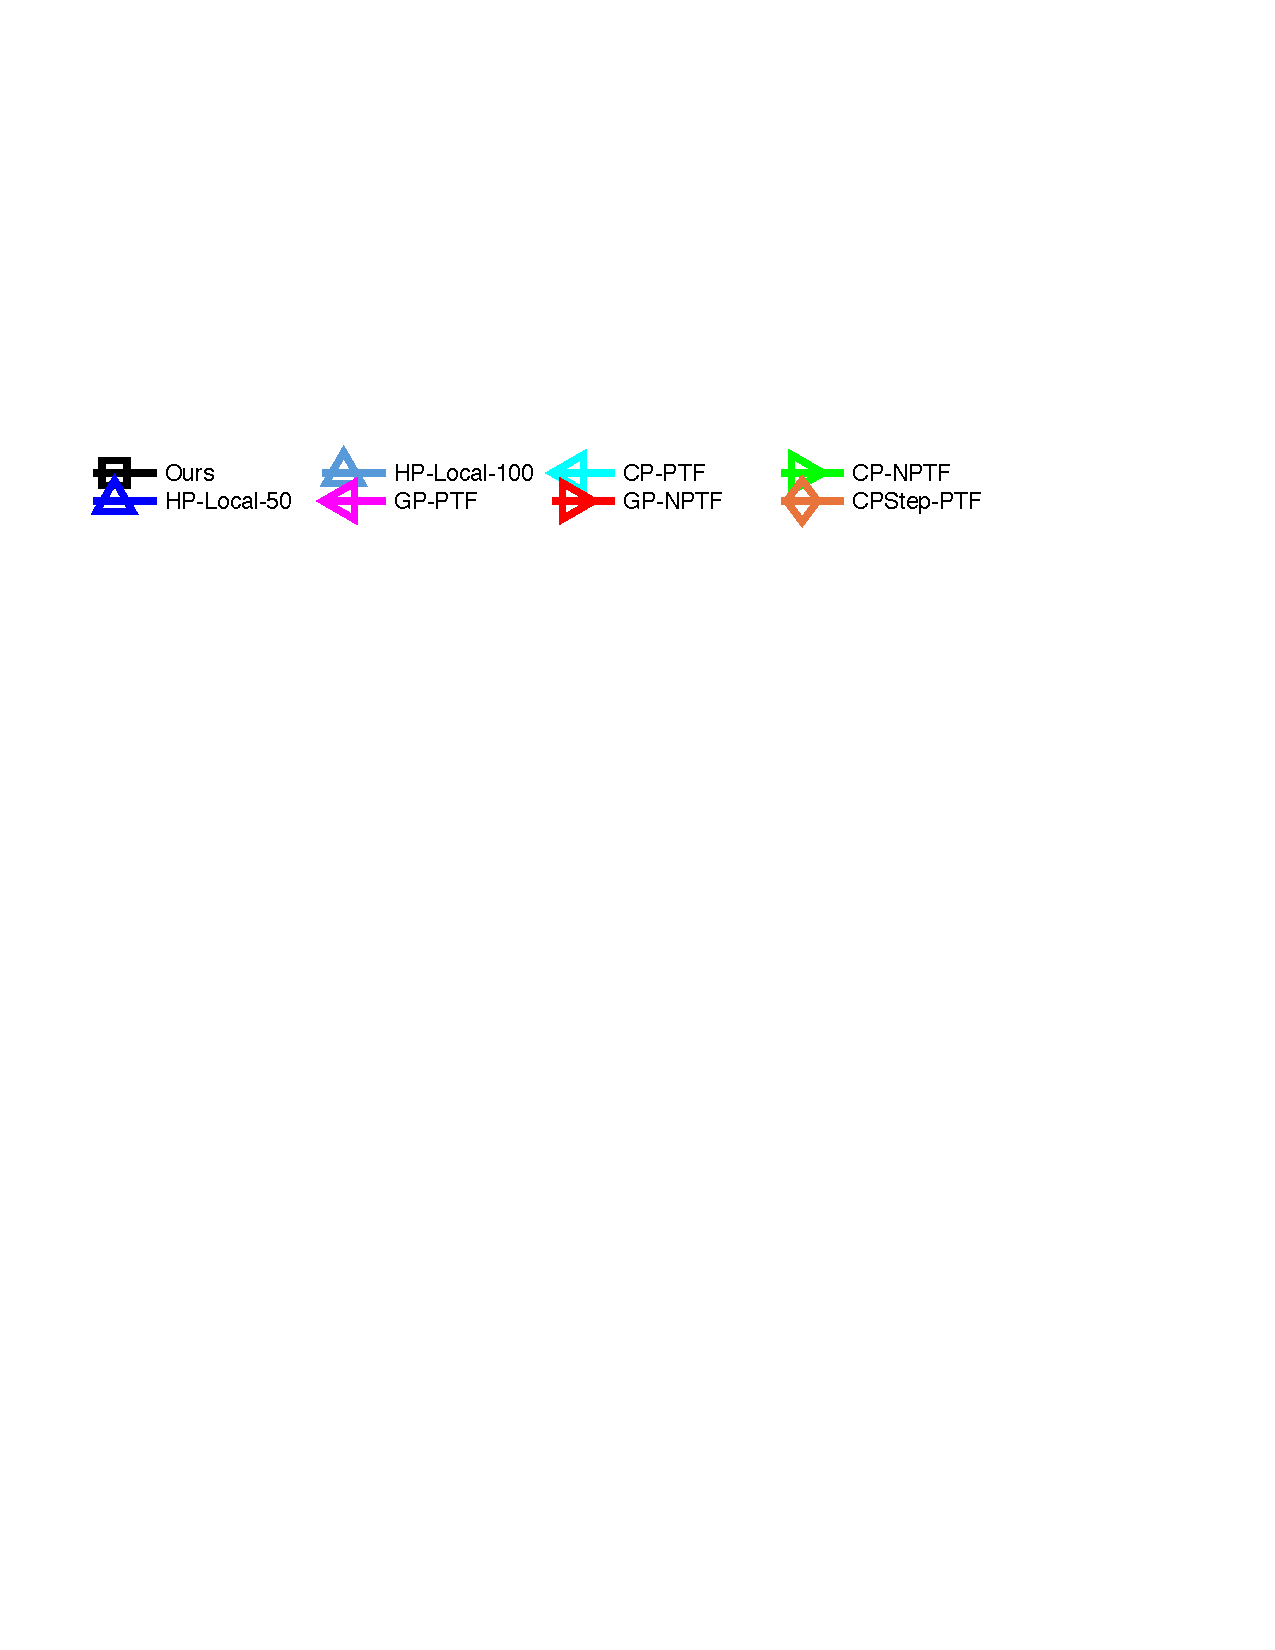
\includegraphics[width=0.618\textwidth]{./figs/ll_legend.pdf}}
		\\
		\begin{subfigure}[t]{0.25\textwidth}
			\centering
			%			\includegraphics[width=\textwidth]{./fig/burger_400_rmse.eps}
			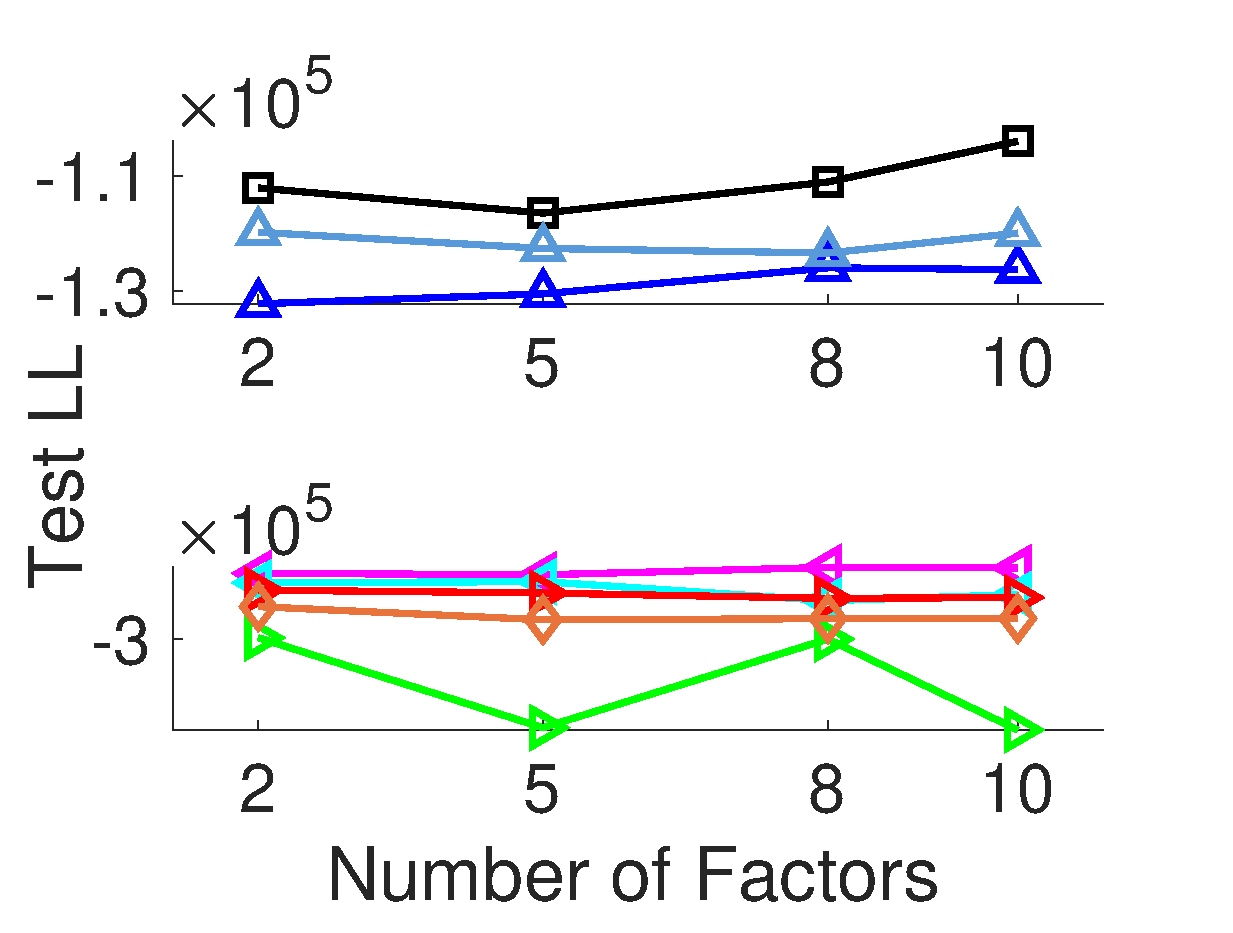
\includegraphics[width=\textwidth]{./figs/taobao_ll.eps}
			\caption{\textit{Taobao}}
		\end{subfigure} 
		&
		\begin{subfigure}[t]{0.25\textwidth}
			\centering
			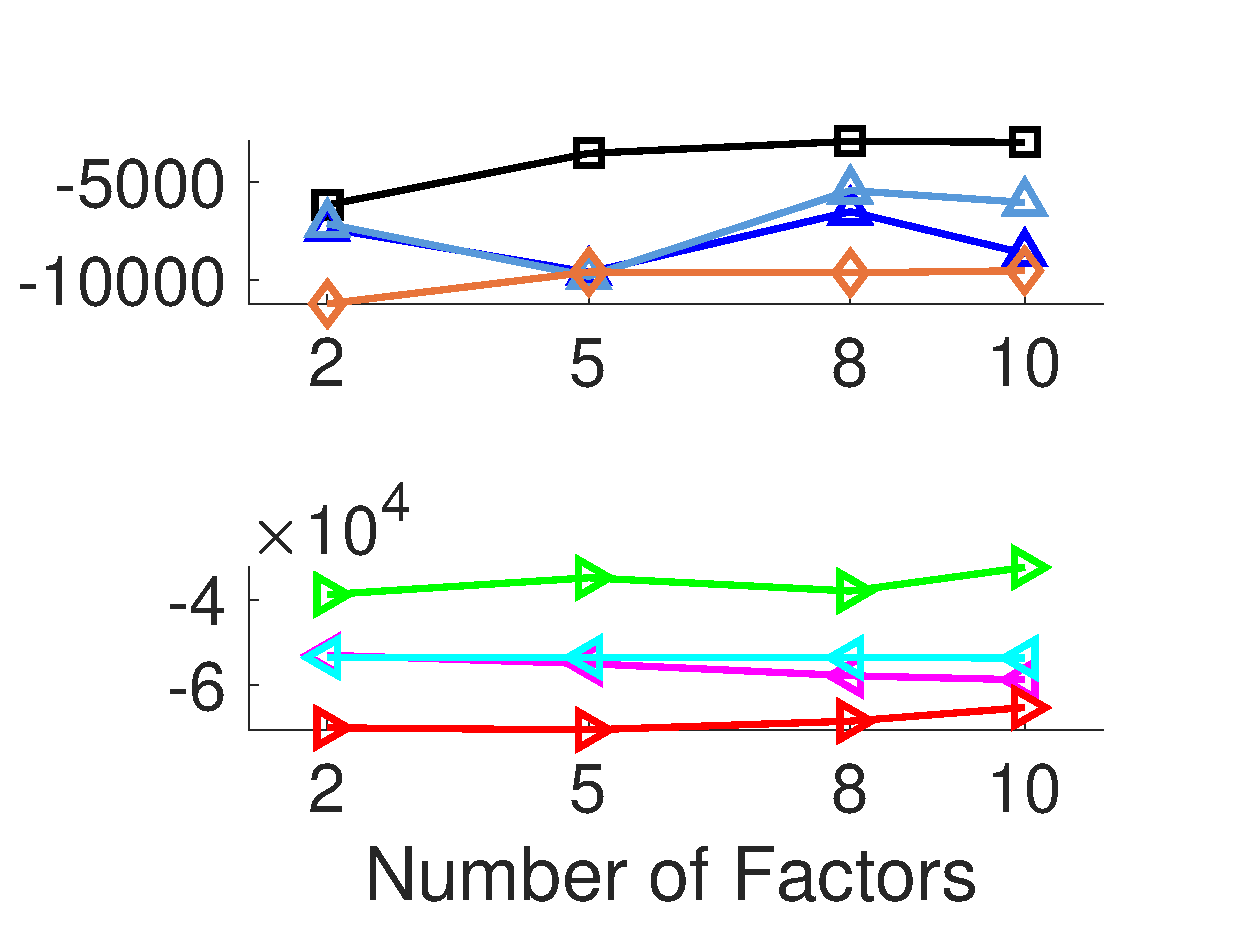
\includegraphics[width=\textwidth]{./figs/ufo_ll.eps}
			\caption{\textit{UFO}}
		\end{subfigure}
		&
		\begin{subfigure}[t]{0.25\textwidth}
			\centering
			%			\includegraphics[width=\textwidth]{./fig/heat_400_rmse.eps}
			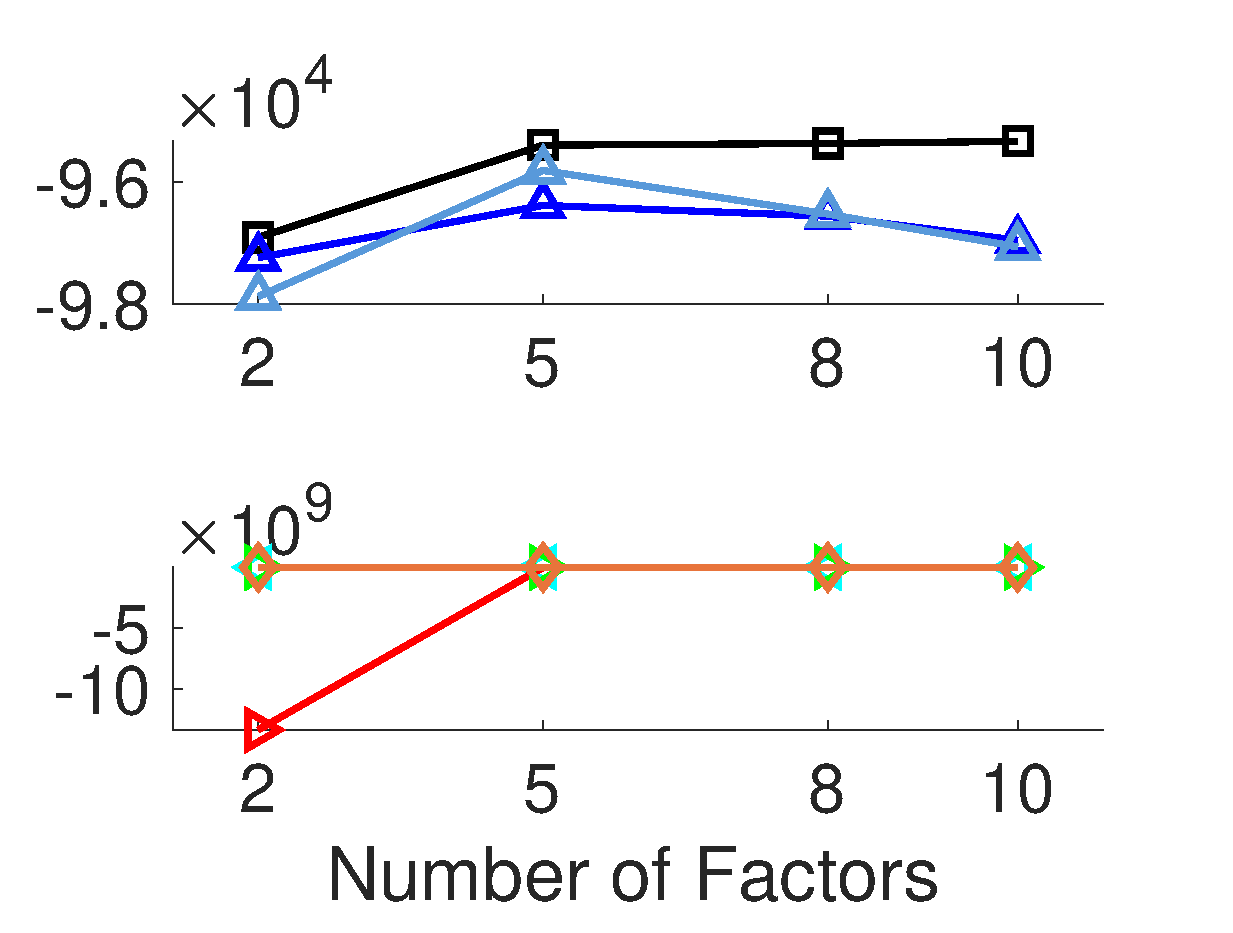
\includegraphics[width=\textwidth]{./figs/crash_ll.eps}
			\caption{\textit{Crash}}
		\end{subfigure} 
		&
		\begin{subfigure}[t]{0.25\textwidth}
			\centering
			%			\includegraphics[width=\textwidth]{./fig/heat_400_rmse.eps}
			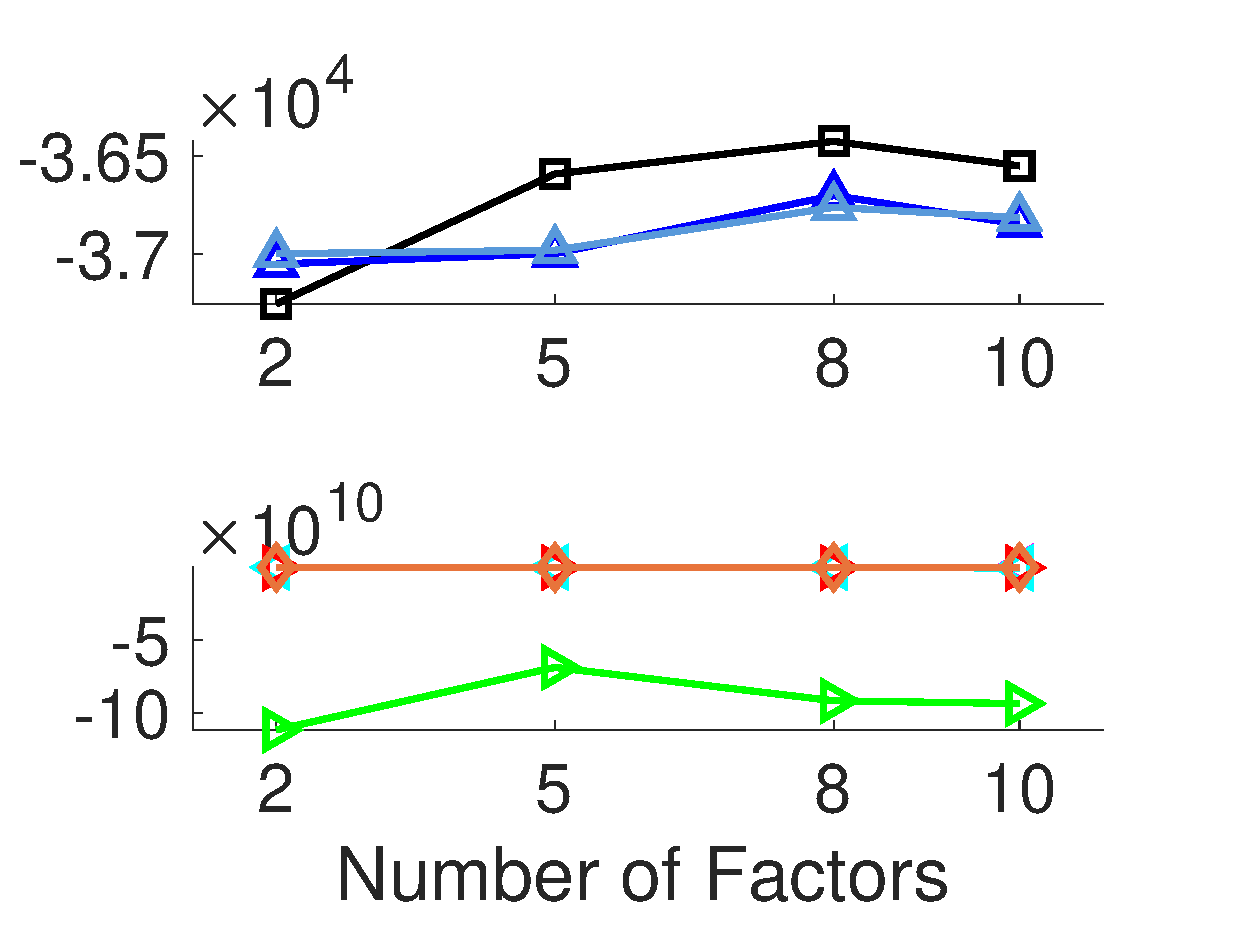
\includegraphics[width=\textwidth]{./figs/lastfm_ll.eps}
			\caption{\textit{LastFM}}
		\end{subfigure} \cmt{\\
		\begin{subfigure}[t]{0.25\linewidth}
			\centering
			%			\includegraphics[width=\textwidth]{./fig/burger_400_rmse.eps}
			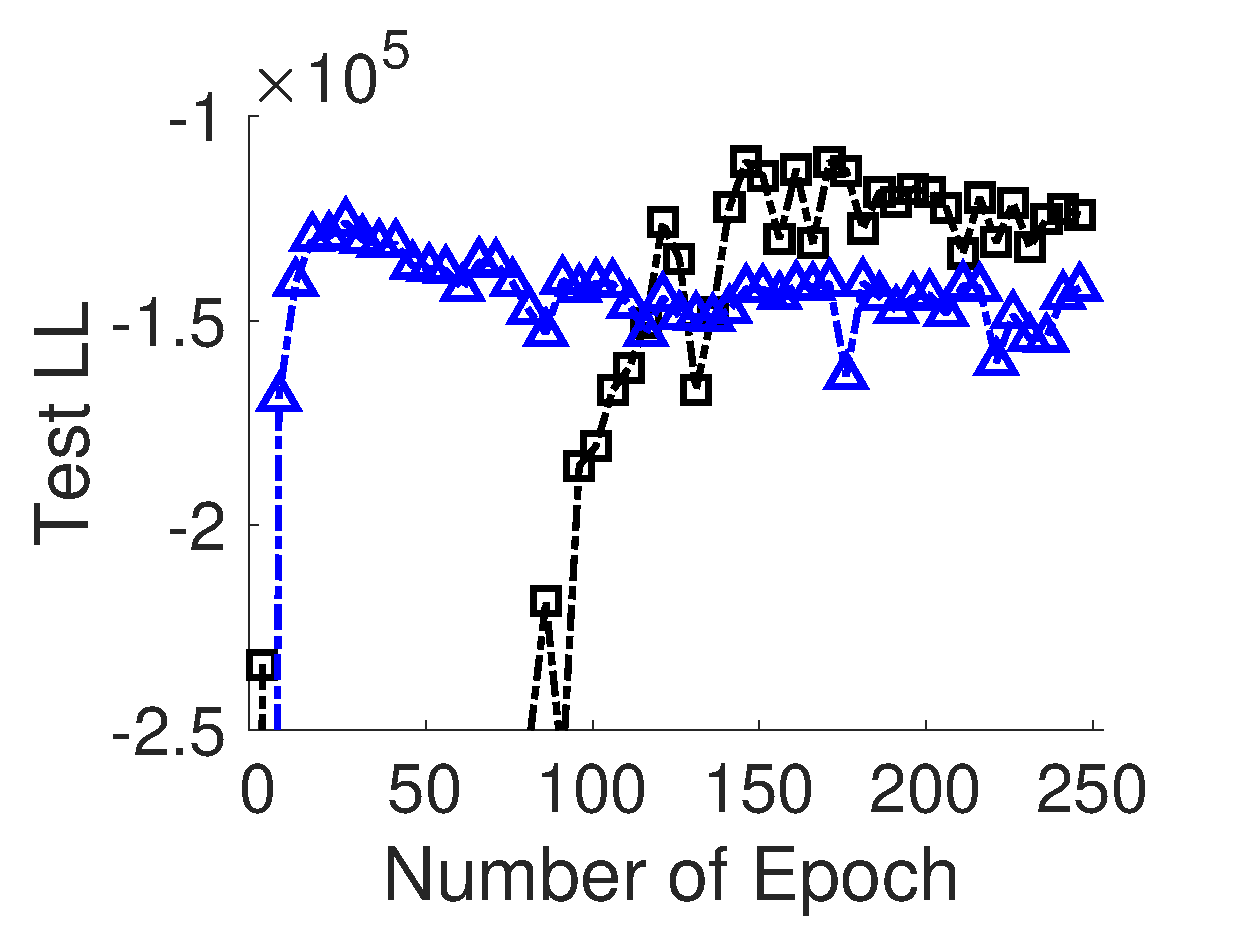
\includegraphics[width=\linewidth]{./figs/taobao_ll_epoch.eps}
			\caption{\textit{Taobao}}
		\end{subfigure} 
		&
		\begin{subfigure}[t]{0.25\linewidth}
			\centering
			%			\includegraphics[width=\textwidth]{./fig/burger_400_rmse.eps}
			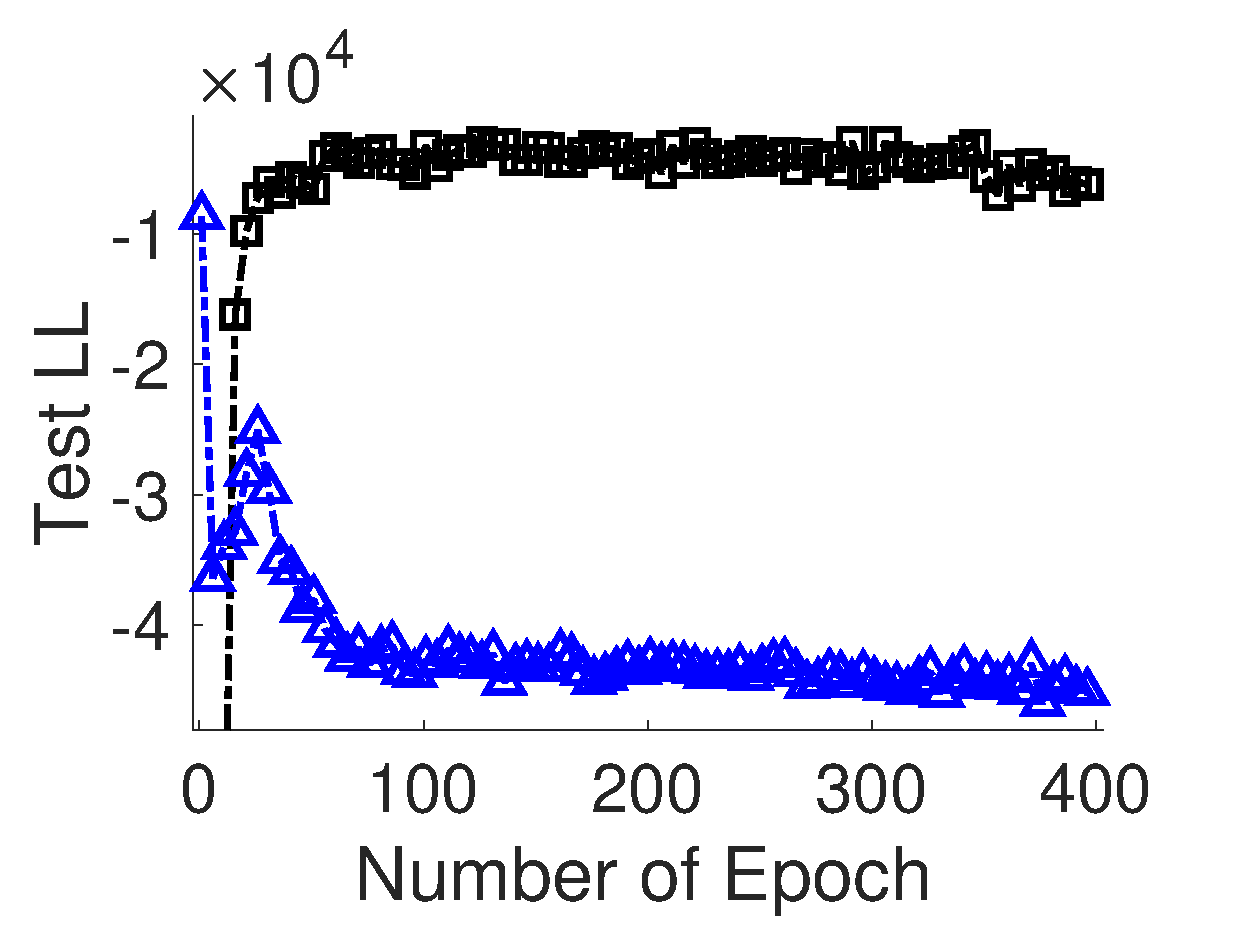
\includegraphics[width=\linewidth]{./figs/ufo_ll_epoch.eps}
			\caption{\textit{UFO}}
		\end{subfigure} 
		&
		\begin{subfigure}[t]{0.25\linewidth}
			\centering
			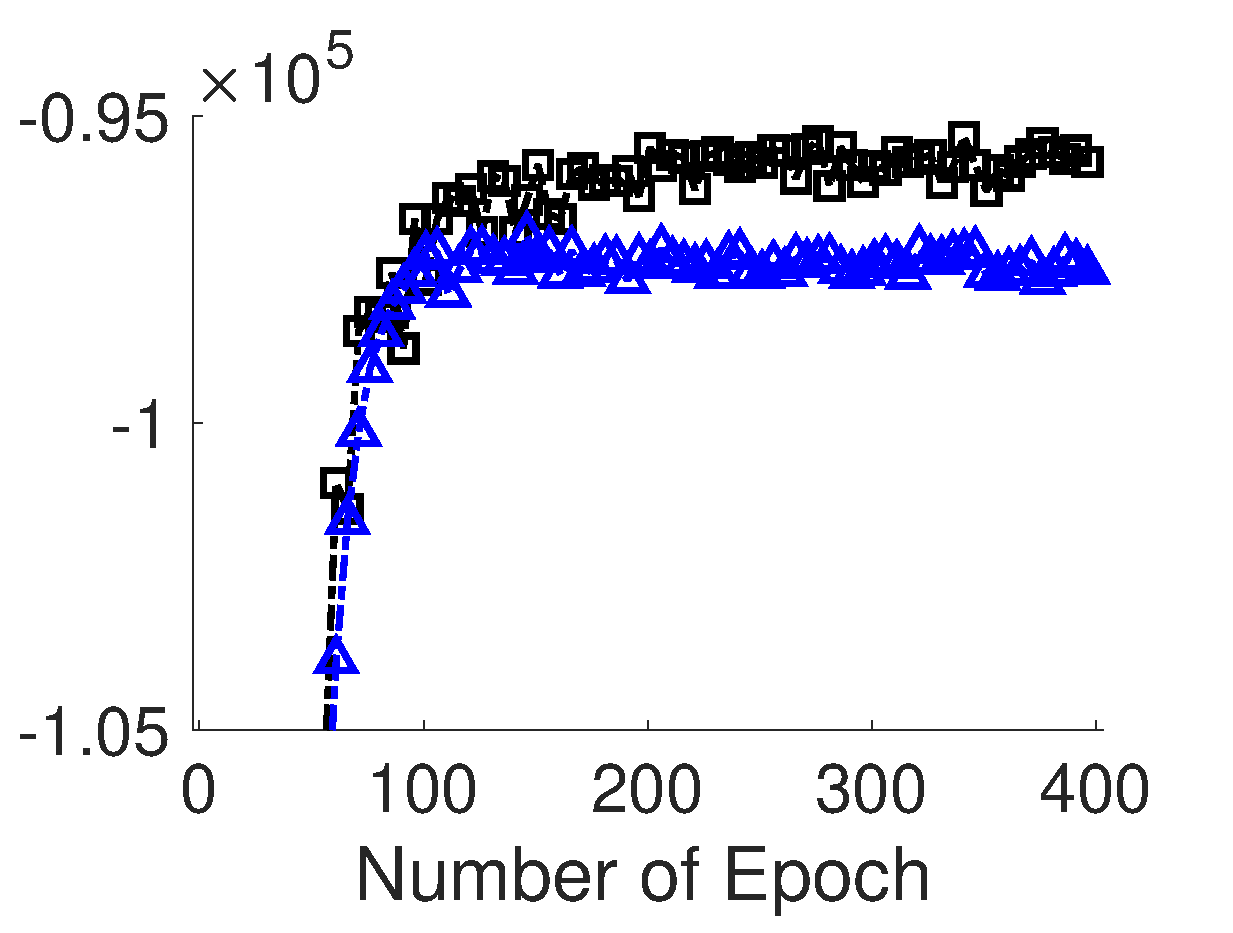
\includegraphics[width=\linewidth]{./figs/crash_ll_epoch.eps}
			\caption{\textit{Crash}}
		\end{subfigure}
		&
		\begin{subfigure}[t]{0.25\linewidth}
			\centering
			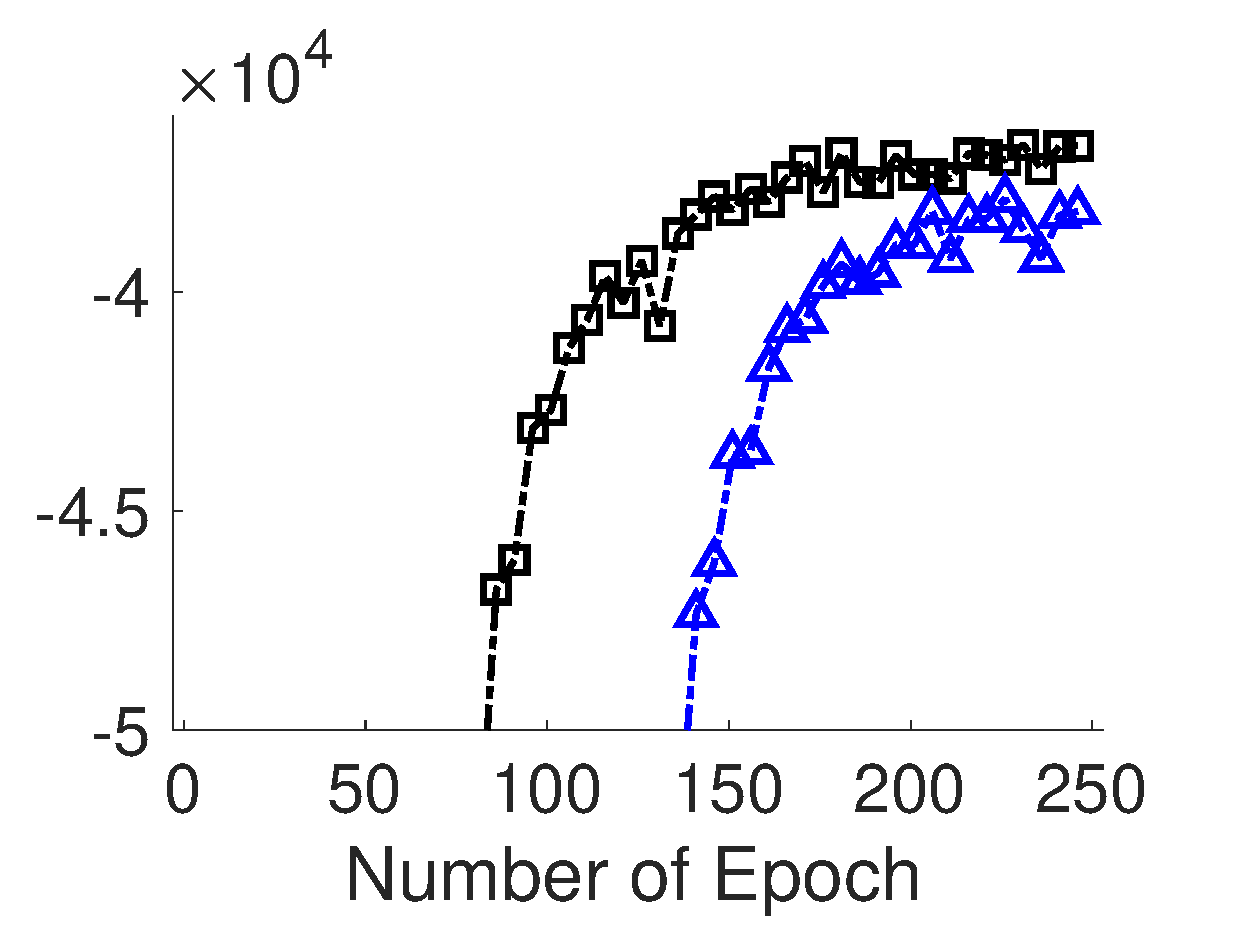
\includegraphics[width=\linewidth]{./figs/lastfm_ll_epoch.eps}
			\caption{\textit{LastFM}}
		\end{subfigure}
	}
	\end{tabular}
	\vspace{-0.1in}
	\caption{Test log likelihood on each dataset with different number of latent factors. HP-Local-\{50, 100\} means running HP-Local with window size $50$ and $100$. The sub-figures on the top include the results only for our method and HP-Local, except that in (b), CPStep-PTF is also included. All the remaining methods are shown in the bottom sub-figures and their performance are much worse. Note that the test log likelihoods of several baselines are very close on \textit{Crash} and  \textit{LastFM} and so their curves overlap. } 	
	\label{fig:test-ll}
	\vspace{-0.2in}
	%\vspace{-0.14in}
\end{figure*}
\textbf{Datasets}. We first examined the predictive performance of our approach on the following four real-world datasets.  (1) \textit{Taobao} (\url{https://tianchi.aliyun.com/dataset/dataDetail?dataId=53}), online shopping behaviours between 07/01/2015 and 11/30/2015 in the largest retail platforms of China. We extracted a $5$-mode tensor, of size $980 \times 274 \times  631 \times  58 \times  2$, which represents the interactions of  \textit{(user, seller, item, category, action)}. The action can be either ``buy'' or ``click''. The number of observed events are $69,833$ where there are $16,609$ distinct interactions (\ie entries). 
   (2) \textit{UFO}~\citep{zhe2018stochastic}, the UFO sighting reports in 20th century. The dataset is a two-mode event-tensor \textit{(UFO shape, city)}, of size $28  \times 13,713$, including $45,045$ observed entries and $70,418$ sighting events. (3) \textit{Crash} (\url{https://www.kaggle.com/usdot/nhtsa-traffic-fatalities}), the report of fatal traffic crashes in US, year 2015. We extracted a $4$-mode tensor \textit{(state, county, city, landuse-type)}, of size $51 \times 288 \times 2,098 \times 5$. 
Each entry consists of a sequence of crash events. There are $8,691$ entries and $32,052$ events in total.  (4) \textit{LastFM} (\url{https://grouplens.org/datasets/hetrec-2011/}), a music tagging dataset. From the most active users, popular artists and tags, we extracted a three-mode event-tensor, \textit{(user, artist, tag)}, of size is $191 \times 200 \times 184$. The tensor has $13,399$ observed entries and the same number of events. That means each interaction occurred only once.  
%The tensor has $13,399$ distinct entries and $13,399$ observed tagging events. 
%92,800 artist listening records from 1892 users. Among all users, artists and music tags, we tried to extract the most active 200 identities for each dimension and got a three mode tensor of size $191  \times 200 \times  184$ where $13399$ events are observed.

\textbf{Competing Methods.}  We compared with the following popular and/or state-of-the-art tensor factorization methods incorporating the temporal information. 
(1) CP-PTF, the homogeneous Poisson process (PP) tensor factorization, which uses CP to factorize the event rate of each entry.  To obtain non-negative rates, we conducted the factorization in the log domain. (2) CPStep-PTF, which is similar to ~\citep{schein2015bayesian}. It discretizes the timestamps into $5$ steps and adds a time mode to the tensor. Time factors are introduced to represent each step and jointly estimated with the other factors. CP is applied to factorize the event rates of each entry in the log domain. (3) GP-PTF, which uses GPs to estimate the log rate of each entry as a nonlinear function of the associated latent factors. This is the same as our approach in modeling the base rate. (4) CP-NPTF, non-homogeneous Poisson process tensor factorization where the event rate is modelled as $\lambda_{\bi}(t) =t\cdot  \exp\big(\mathrm{CP(\bi)}\big) $ for each $\bi$. Here $\mathrm{CP}(\bi)$ is CP factorization of entry $\bi$. (5) GP-NPTF, non-homogeneous PP tensor factorization that replaces CP with GP in the rate modeling for CP-NPTF. (6) HP-Local~\citep{zhe2018stochastic}, Hawkes process event-tensor decomposition using a local time window to define the rate function and to estimate the local triggering effects among the neighbouring events.

%how we do
\textbf{Experimental settings.}  For all the competing methods that use GPs, we applied the same sparse GP framework as in our method for scalable inference: we set the number of pseudo inputs to $100$ and used SE-ARD kernel for which we initialized all the parameters to $1$. For a fair comparison, all the methods were initialized with the same set of factors that were independently sampled from $\mathrm{Uniform}(0, 1)$. We implemented our approach and HP-Local with PyTorch and used ADAM~\citep{kingma2014adam} for stochastic optimization. For both methods, the mini-batch size was set to $100$. The learning rate was chosen from $\{5\times 10^{-4}, 10^{-3}, 3\times 10^{-3}, 5 \times 10^{-3}, 10^{-2}\}$. We ran each method for $400$ epochs, which are sufficient for convergence. All the other methods were implemented with MATLAB.  For training, we used the first 40K, 40K, 20K and 10K events from \textit{Taobao}, \textit{UFO}, \textit{Crash} and \textit{LastFM}, respectively. The remaining 29.8K, 30.4K, 12K and 3.3K events were used for test. %For CPT-PTF, the number of time steps is varied from \{5, 10, 20\}. 
For HP-Local, we varied the window size from $\{50, 100\}$. Note that the event sequences for test are very long, through which we can examine the performance of our method in capturing long-term temporal effects. We varied the number of the latent from $\{2, 5, 8, 10\}$. We calculated the test log-likelihood of each method, and report the results in Figure \ref{fig:test-ll}. 

\begin{figure}
	\centering
	\setlength\tabcolsep{0.01pt}
	\begin{tabular}[c]{cc}
		\begin{subfigure}[t]{0.48\linewidth}
			\centering
			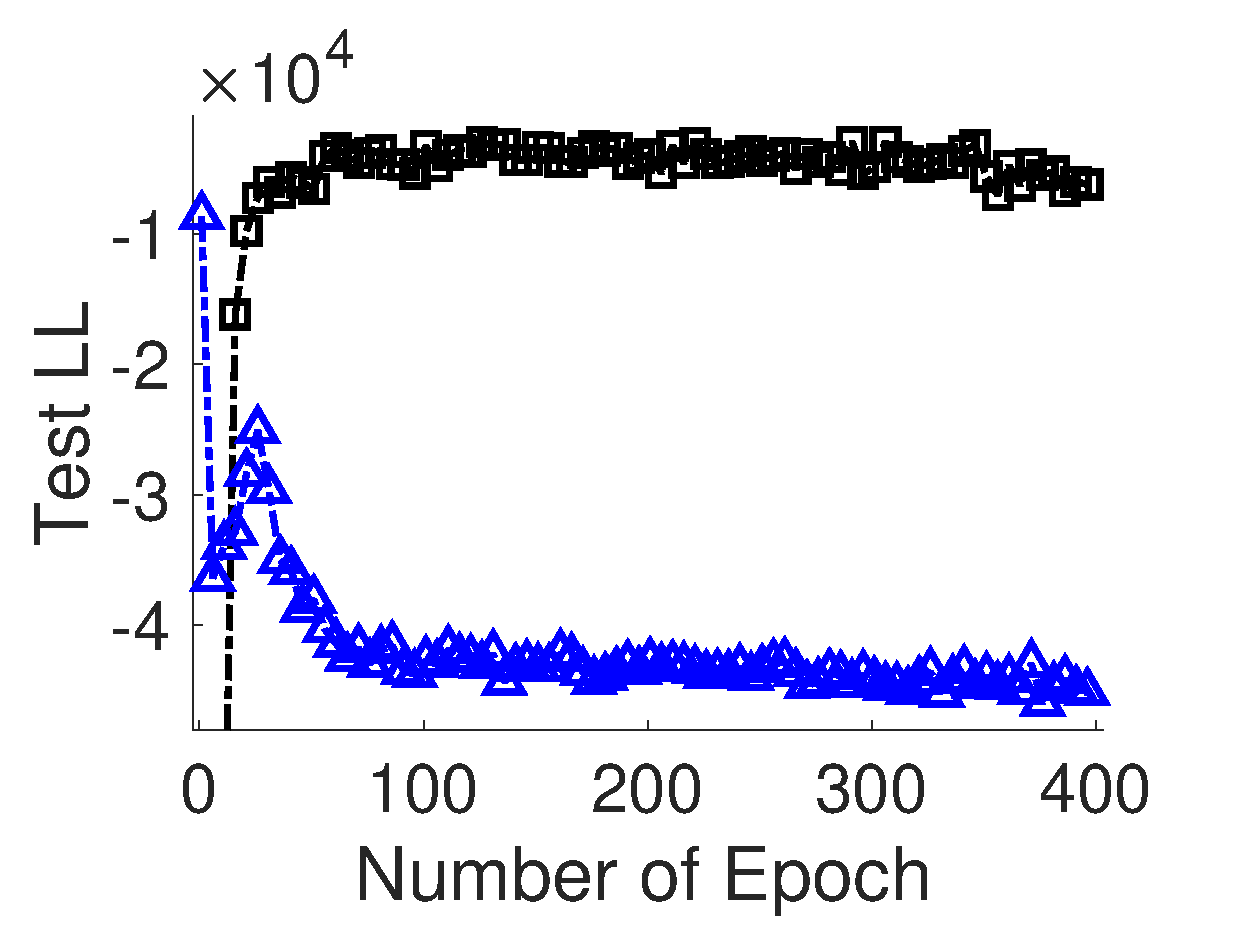
\includegraphics[width=\linewidth]{./figs/ufo_ll_epoch.eps}
			\caption{\textit{UFO}}
		\end{subfigure} 
		&
		\begin{subfigure}[t]{0.48\linewidth}
			\centering
			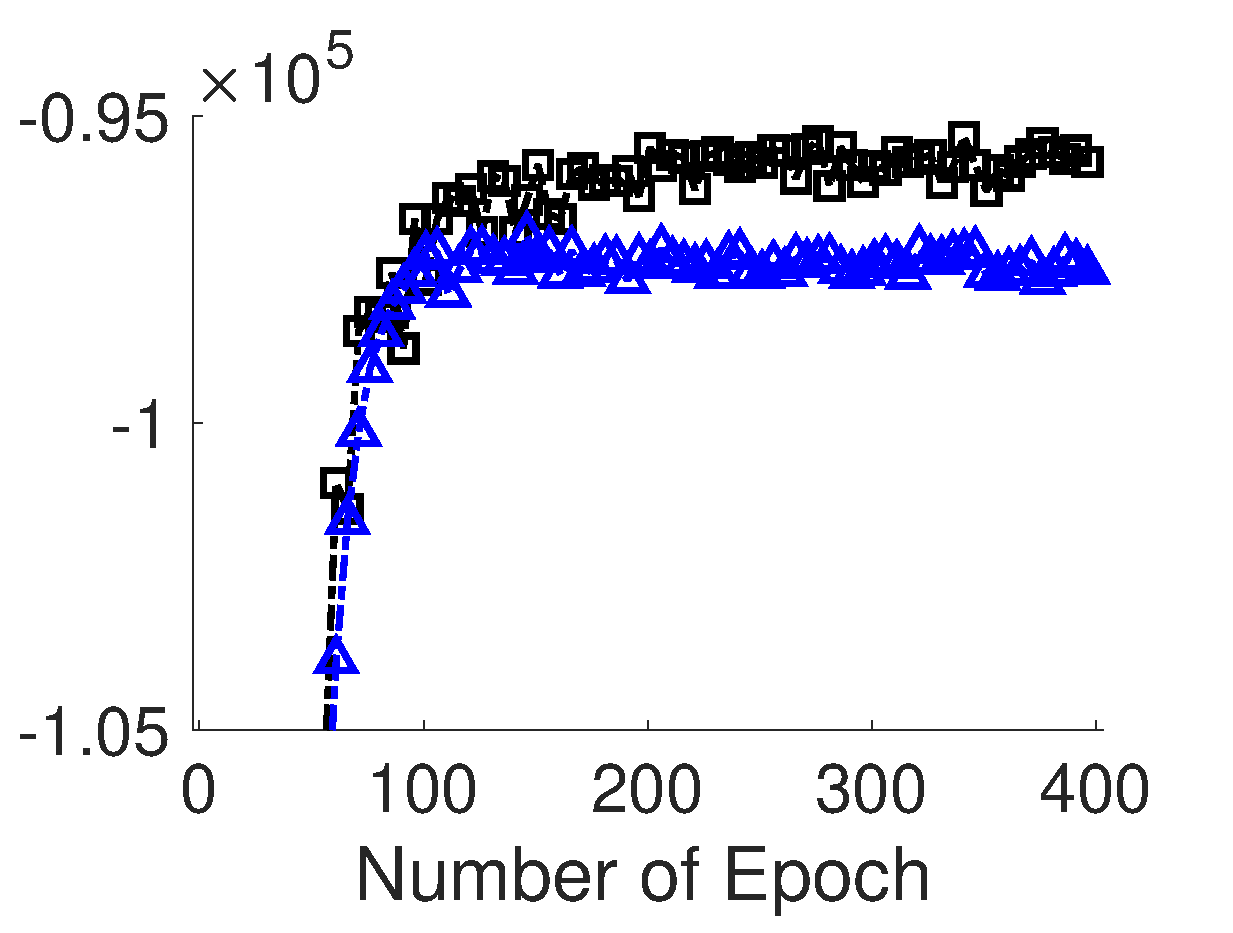
\includegraphics[width=\linewidth]{./figs/crash_ll_epoch.eps}
			\caption{\textit{Crash}}
		\end{subfigure}
	\end{tabular}
\vspace{-0.1in}
\caption{\small The test log likelihood of our method and HP-Local-50 along with the number of training epochs.} 	
\label{fig:learn-curve}
\vspace{-0.3in}
\end{figure}
\begin{figure*}
	\centering
	\setlength\tabcolsep{0.01pt}
	\begin{tabular}[c]{ccc}
		\raisebox{0.8in}{
			\begin{tabular}[c]{c}
				\begin{subfigure}[t]{0.23\textwidth}
					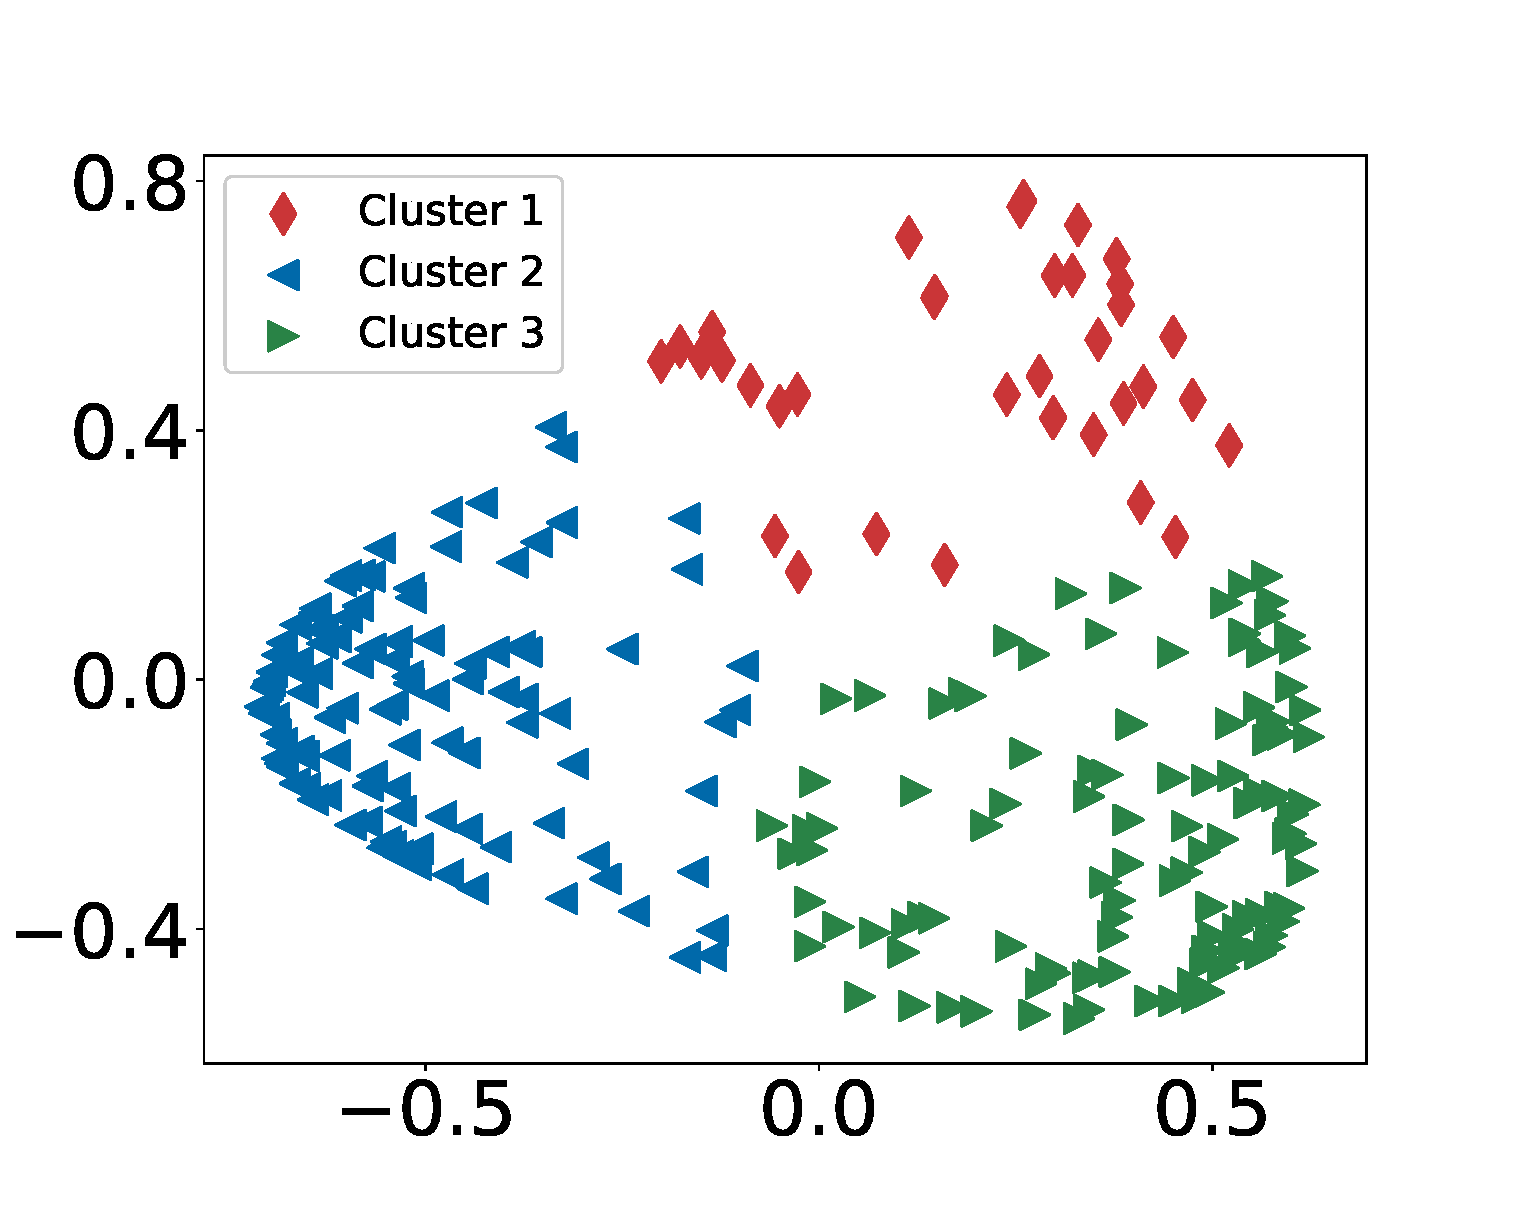
\includegraphics[width=\textwidth]{./figs/taobao_seller_cluster_scatter.eps}
					\caption{\textit{Sellers}}
				\end{subfigure}
				\\
				\begin{subfigure}[t]{0.23\textwidth}
					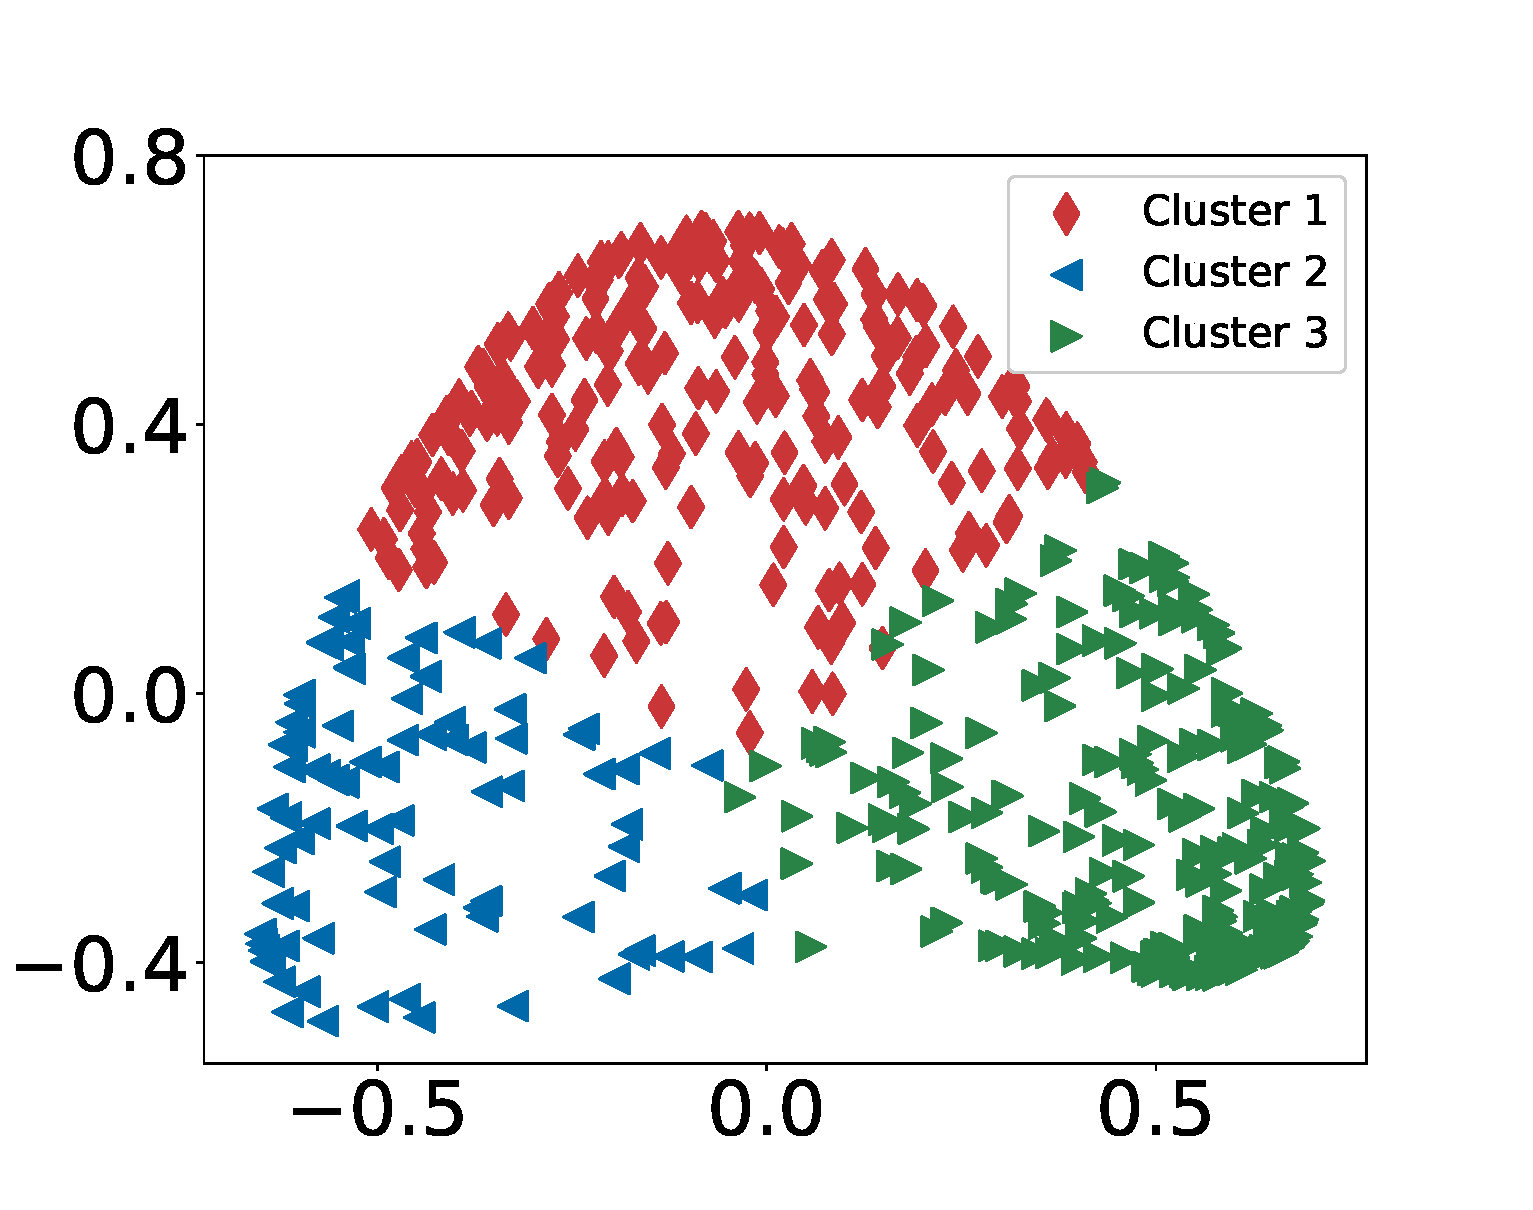
\includegraphics[width=\textwidth]{./figs/taobao_item_cluster_scatter.eps}
					\caption{\textit{Items}}
				\end{subfigure}
			\end{tabular} 
		} &
		\raisebox{0.8in}{
			\begin{tabular}[c]{c}
				\begin{subfigure}[t]{0.23\textwidth}
					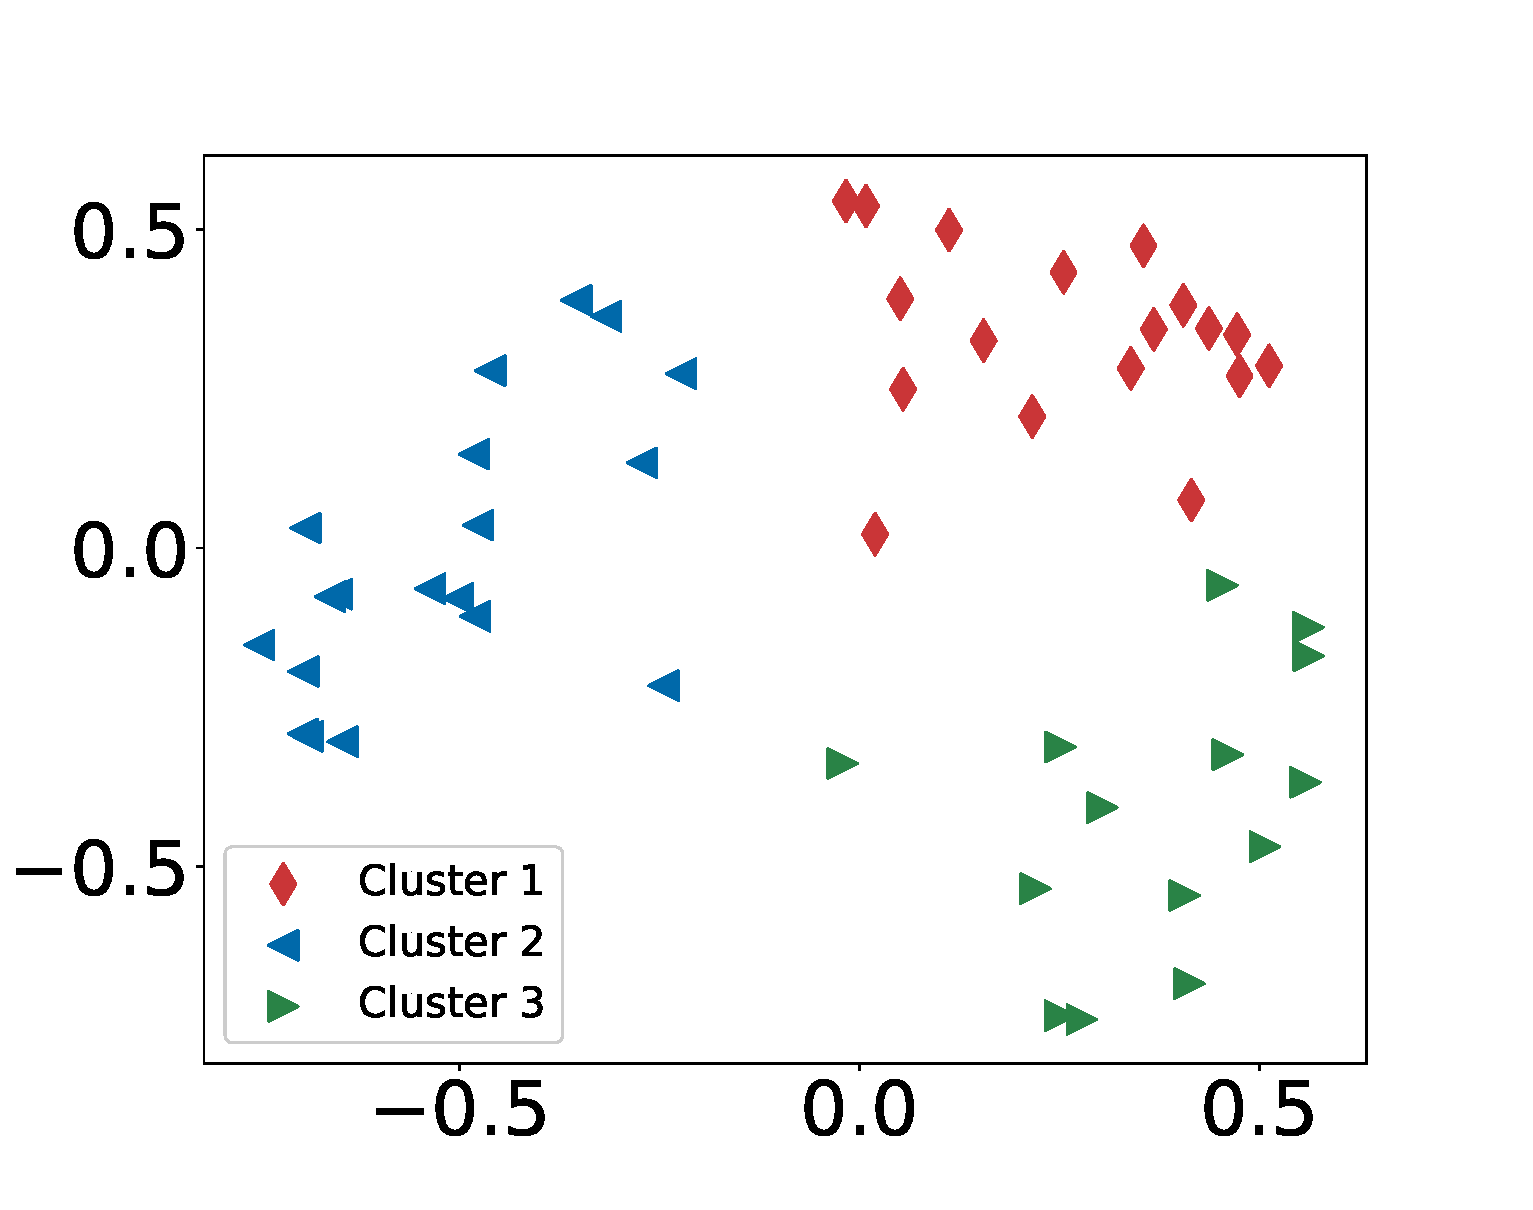
\includegraphics[width=\textwidth]{./figs/SMIE-structure/crash_state_cluster_scatter.eps}
					\caption{\textit{States}}
				\end{subfigure}
				\\
				\begin{subfigure}[t]{0.23\textwidth}
					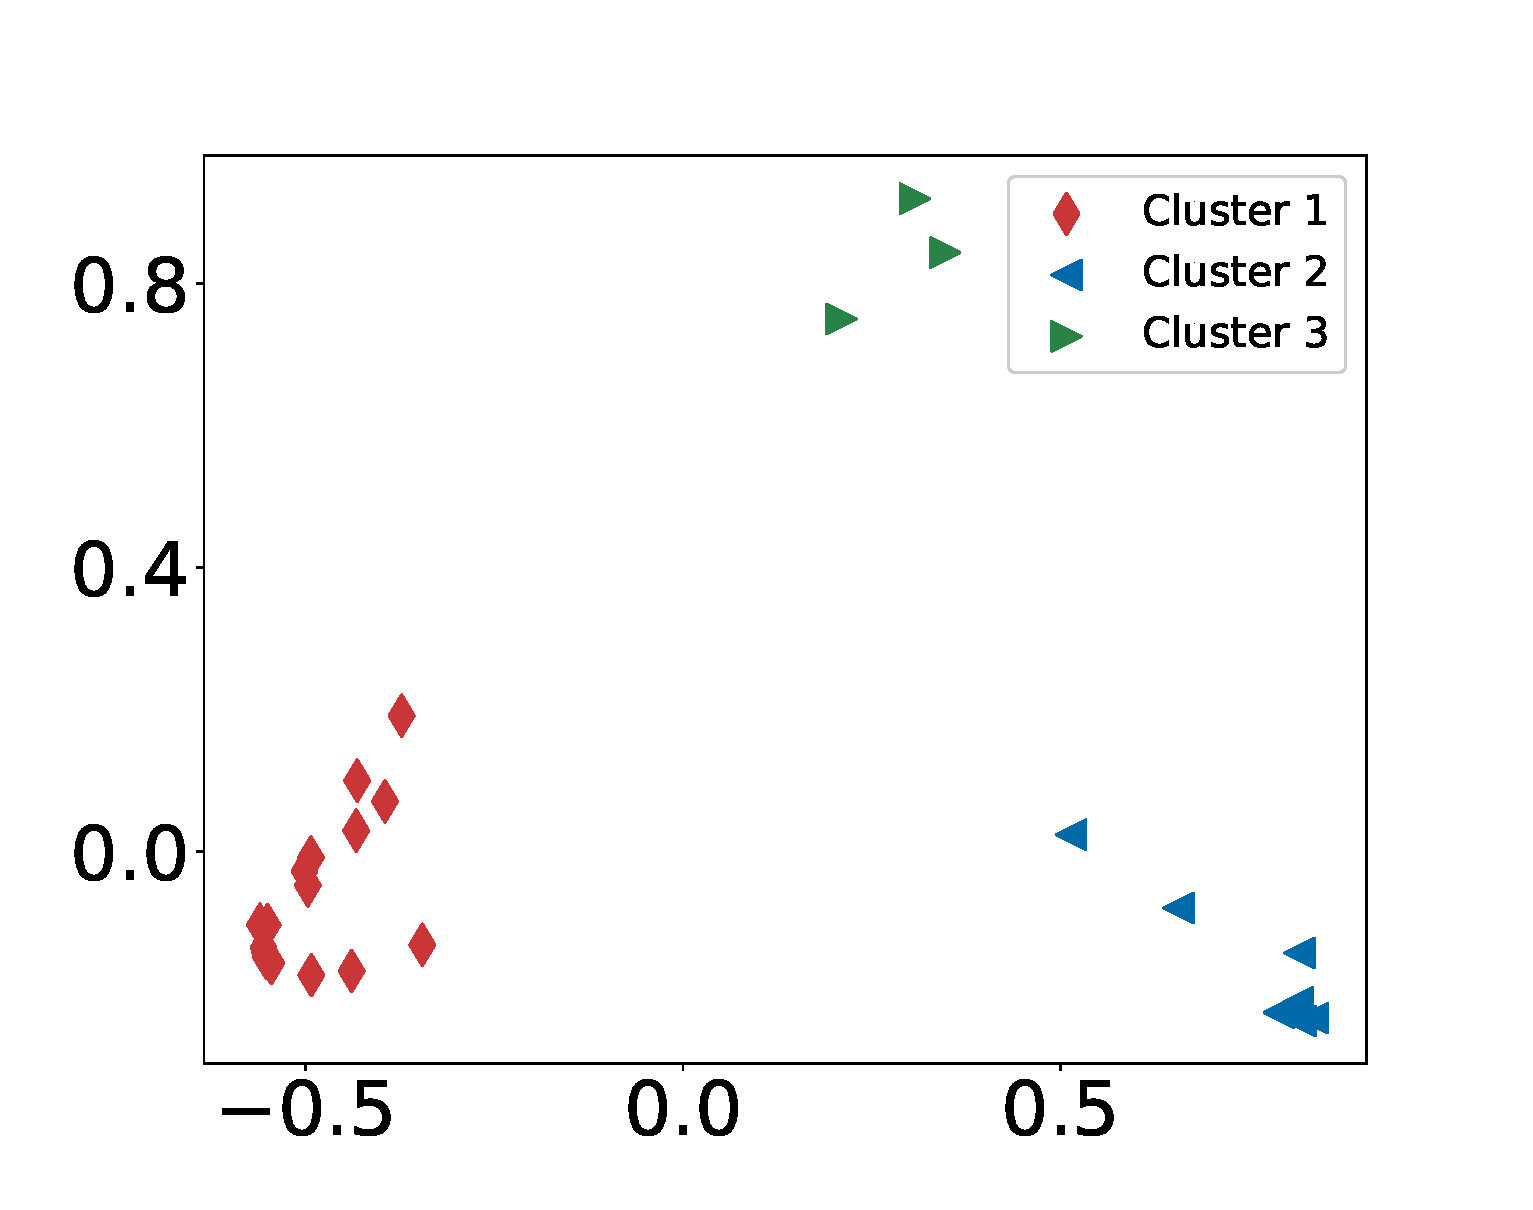
\includegraphics[width=\textwidth]{./figs/ufo_shape_cluster_scatter.eps}
					\caption{\textit{UFO shapes}}
				\end{subfigure}
			\end{tabular} 
		}
		&
		\begin{subfigure}[t]{0.4\textwidth}
			\centering
			\includegraphics[width=\textwidth]{./figs/SMIE-structure/crash-2015-state-trim.pdf}
			\caption{Geolocations of the state clusters}
		\end{subfigure}
	\end{tabular}
\vspace{-0.15in}
	\caption{\small Structures reflected from the latent factors learned by our model on \textit{Taobao} (a, b), \textit{Crash} (c, e) and \textit{UFO} (d). Colors indicate cluster memberships.}\label{fig:crash-ufo}
	\vspace{-0.2in}
\end{figure*}
\textbf{Results.} As we can see from Fig. \ref{fig:test-ll}, our approach consistently outperforms all the competing method except that on \textit{LastFM}, our method is a bit worse than HP-Local when the number of latent factors is $2$. The results demonstrate the advantage of our method in terms of predictive performance. Note that in general, when we increased the window size, HP-Local obtained better or similar prediction accuracy (\eg Fig. \ref{fig:test-ll}a); hence it  shows that estimating long-range temporal dependencies can help improve the predictive performance.  The other competing methods, \eg CP-PTF, GP-PTF, CP-NPTF and GP-NPTF, are far worse than our model and HP-Local in almost all the cases. For better illustration, we show their test log likelihoods in separate sub-figures at the bottom.  Note that these methods are based on homogeneous or non-homogeneous Poisson processes and disregard the temporal dependencies among the interaction events. Therefore, their results further demonstrate the benefit of our model being capable of capturing various, complex temporal dependencies among the events. 


We then investigated the learning behaviour of our model, as shown in Fig. \ref{fig:learn-curve}. Our learning algorithm converges reasonably fast (around $100$ epochs on both \textit{UFO} and \textit{Crash}), and then keeps stable after the convergence. Hence, there is not an apparent overfitting issue and we do not need to use extra tricks such as early stopping. The reason might be that our training objective \eqref{eq:elbo-3} is a lower bound of the model evidence and can effectively resist overfitting (like many other variational inference algorithms). 
\begin{figure}
	\vspace{-0.1in}
	\centering
	\setlength\tabcolsep{0.01pt}
	\begin{tabular}[c]{cc}
		\begin{subfigure}[t]{0.23\textwidth}
			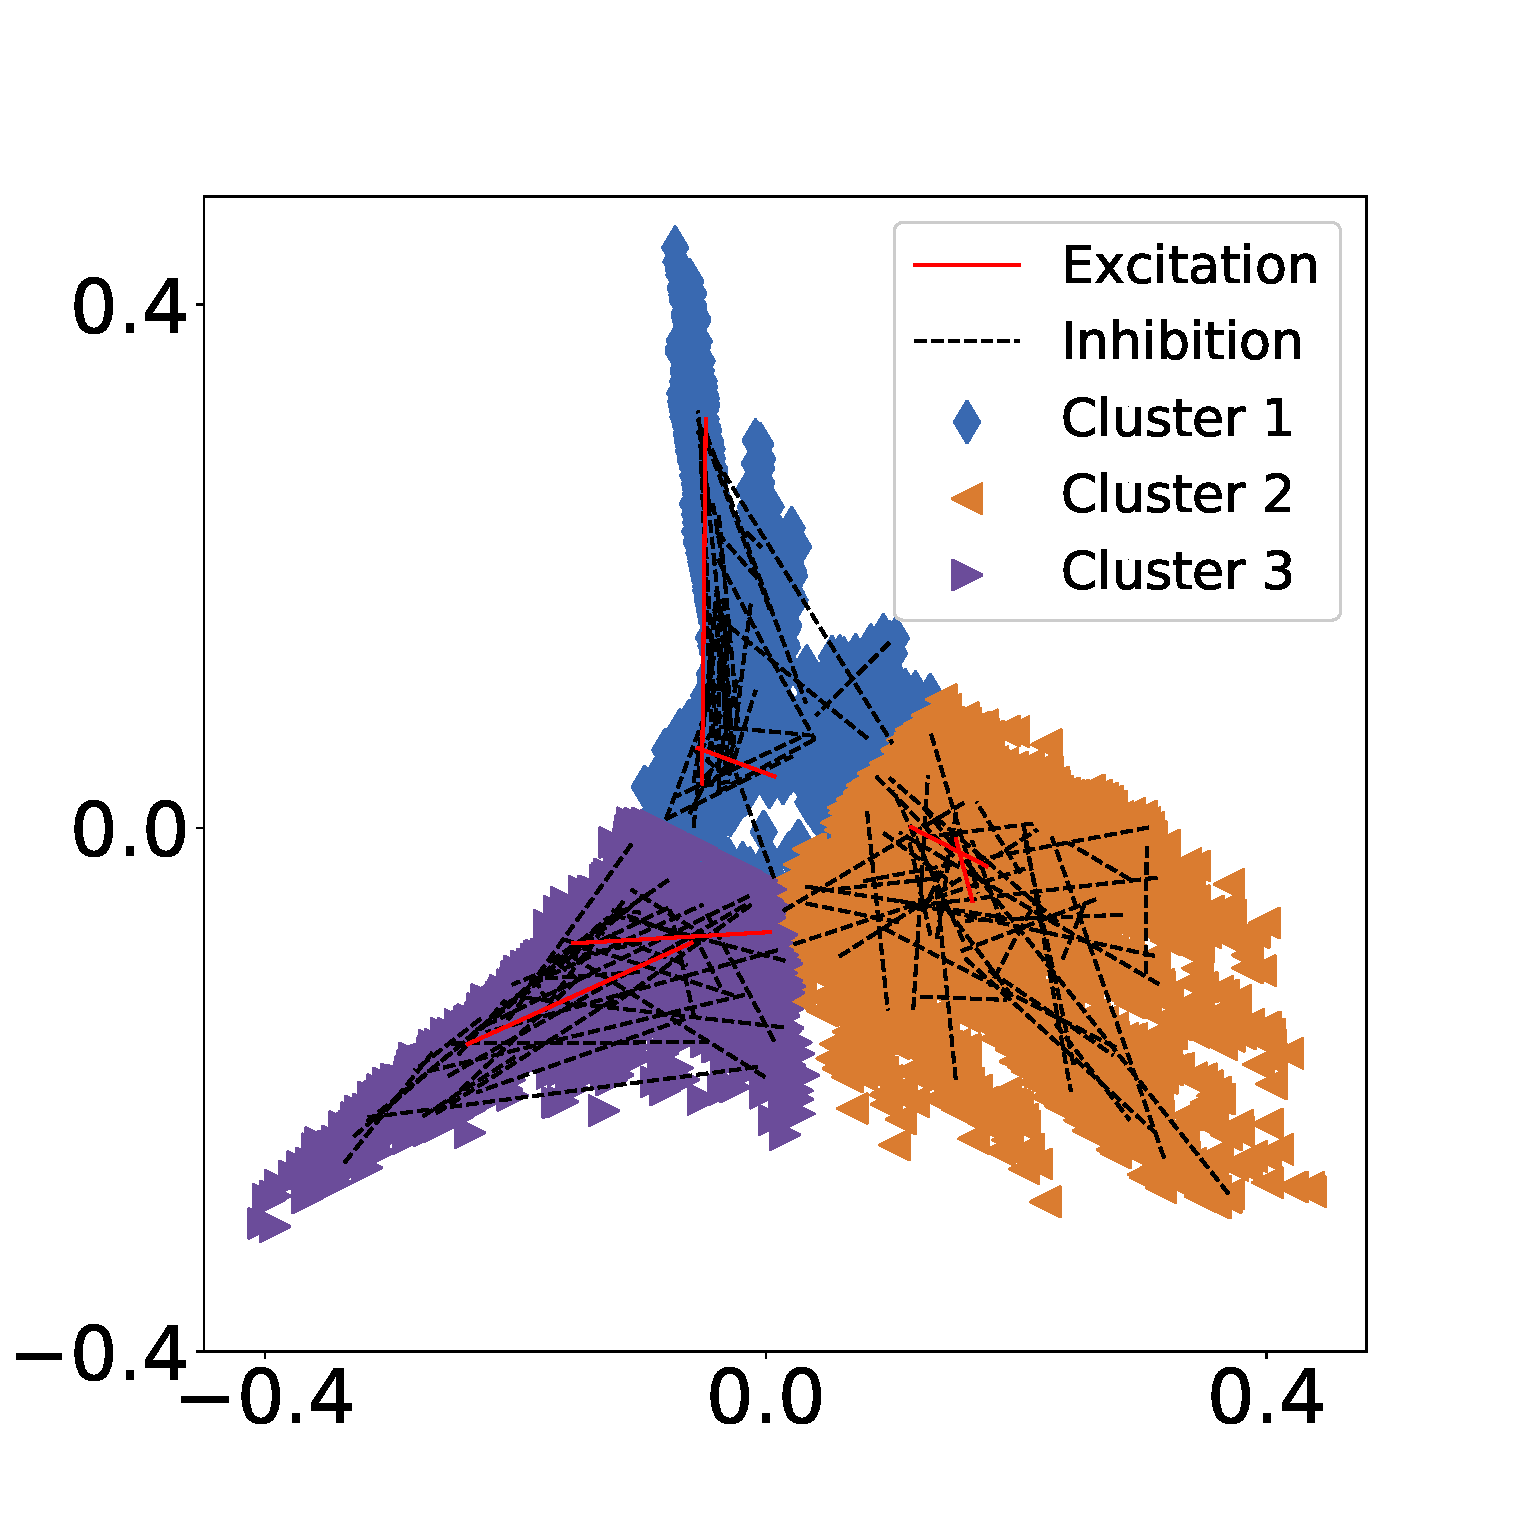
\includegraphics[width=\textwidth]{./figs/lastfm_s3_inner.eps}
			\caption{\textit{Within clusters}}
		\end{subfigure} &
		\begin{subfigure}[t]{0.23\textwidth}
			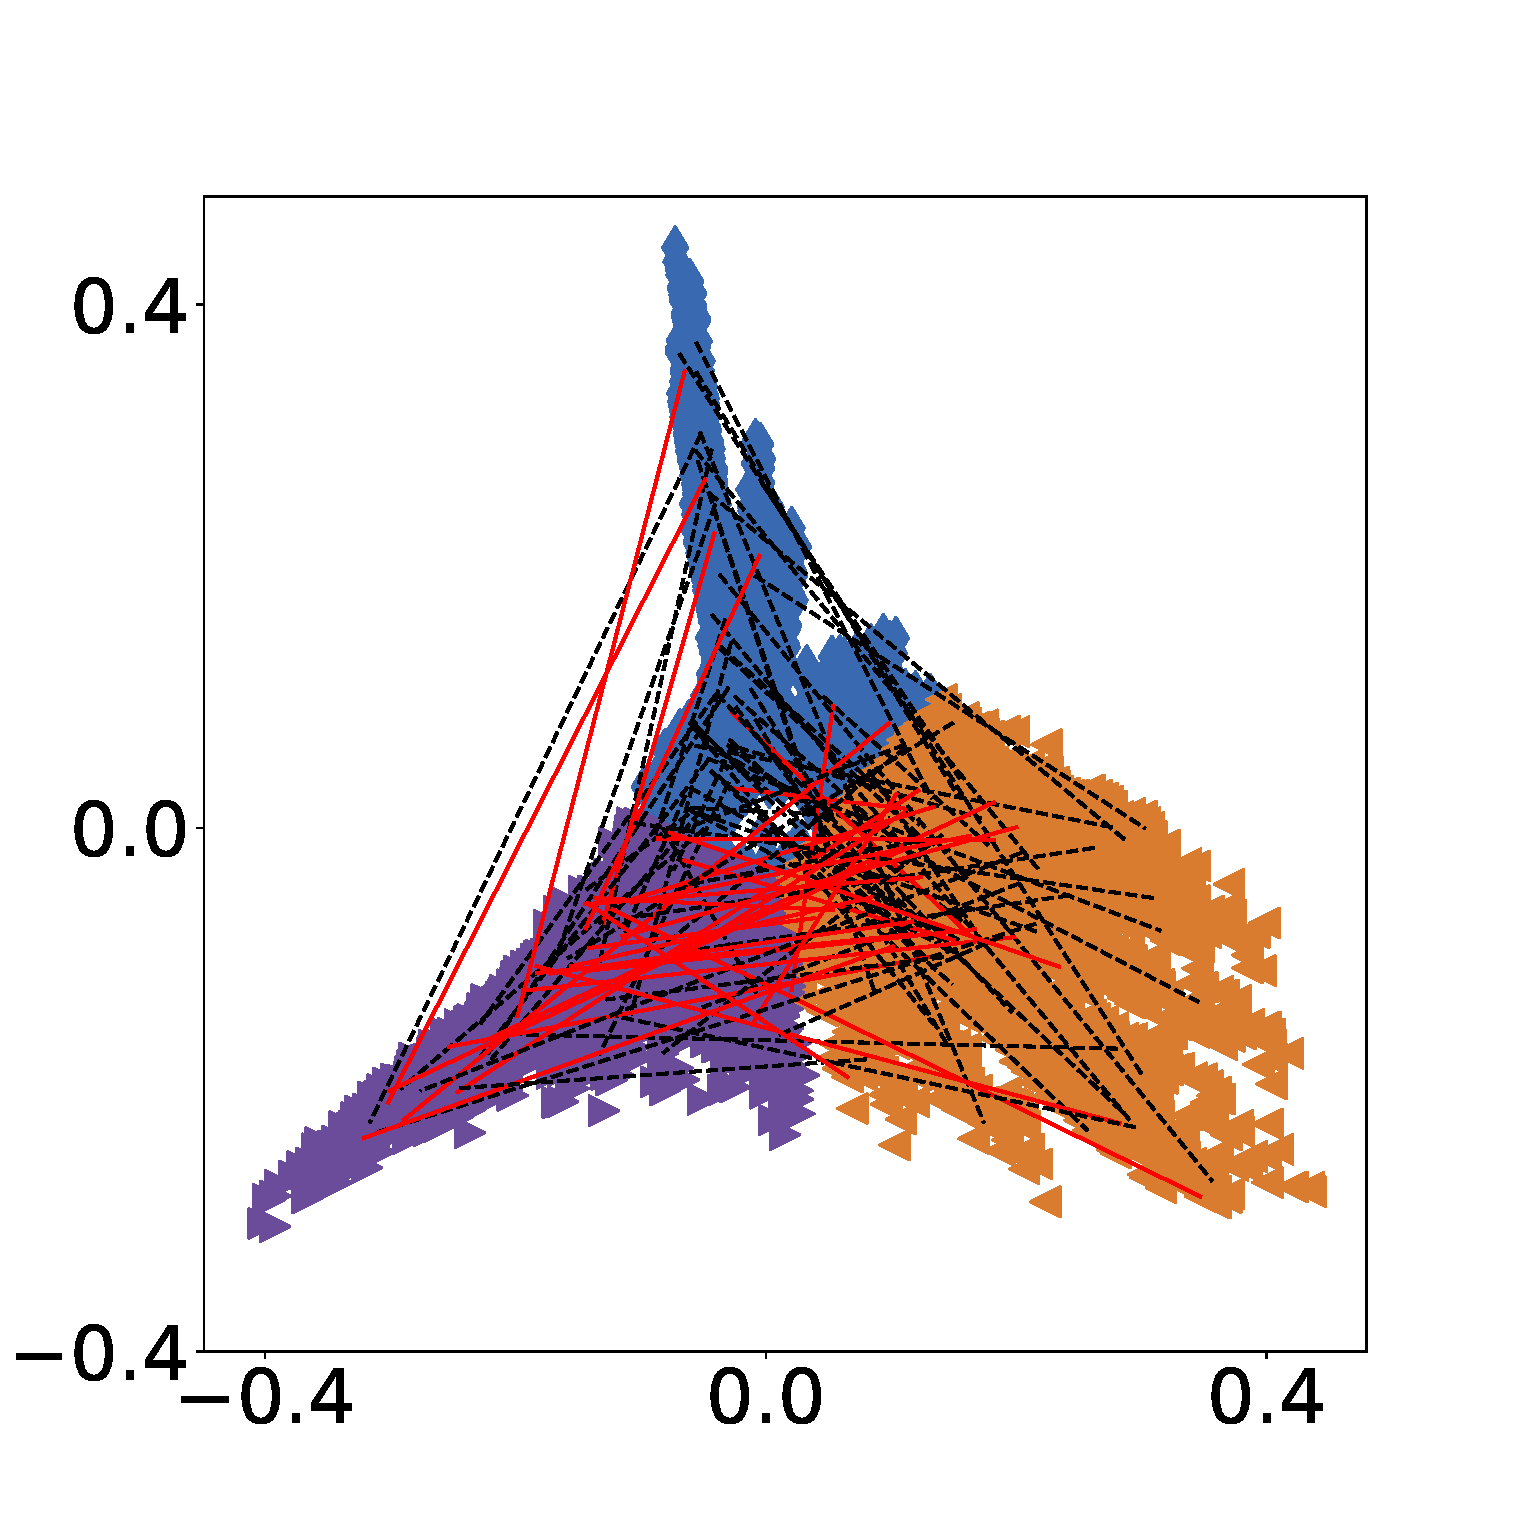
\includegraphics[width=\textwidth]{./figs/lastfm_s3_cross.eps}
			\caption{\textit{Across clusters}}
		\end{subfigure}
	\end{tabular}
\vspace{-0.15in}
	\caption{\small Structures of the events and their temporal influences in \textit{LastFM}.} \label{fig:lastfm} 
	\vspace{-0.3in} 
\end{figure}
\vspace{-0.1in}
\subsection{Structure Discovery}
\vspace{-0.05in}
Next, we examined if our method can discover hidden structures in the data. To this end, we set the number of latent factors to $10$ and ran our algorithm on \textit{Crash}, \textit{UFO} and \textit{Taobao}. Then we applied kernel PCA~\citep{scholkopf1998nonlinear} (with RBF kernel) to project the latent factors onto the x-y plane. We then ran k-means to find the potential clusters in the (projected) factor representations of the entities. We used the elbow method~\citep{ketchen1996application} to select the number of clusters. As we can see from Fig. \ref{fig:crash-ufo}, these factors reflected clear grouping structures. Note that \textit{Taobao} data have been anonymized so we cannot investigate the meaning of those clusters. But they can be potentially useful for tasks like recommendation~\citep{tran2018regularizing} and click-through-rate prediction~\citep{pan2019warm}. Then for \textit{Crash} data, we show the actual geolocations of the clustered states in Figure \ref{fig:crash-ufo}e. We can see that states grouped together are often neighbouring with each other. The clusters can be roughly seen as the middle (red), the south (blue) and the east/west coast (green). This is reasonable --- the states close by may have similar patterns of the traffic crash events and their chain effects (inhibition/excitation) due to similar driving customs, roads layout and weather patterns. 

We also looked into the triggering and inhibition effects among the interaction evens. To this end, we ran our algorithm on \textit{LastFM}. We represented each music tagging event by concatenating the latent factors of participants, \ie the user, artist and tag. We then used kernel PCA to project the event representations onto the x-y plane, and ran k-means to obtain the clusters. We then randomly sample pairs of events within and across clusters, and show their triggering/inhibition relationships with red/black colors. As shown in Fig. \ref{fig:lastfm}a and b, the factor representations of the events present a clear cluster structure. Interestingly, we can see that events within the same cluster mainly inhibit each other (see Fig. \ref{fig:lastfm}a), while across different clusters often excite each other (see Fig. \ref{fig:lastfm}b). This might because users tend to tag artists with distinct/orthogonal styles, rather than keep tagging the same types of artists with very close tags/labels. 


\vspace{-0.1in}
\section{Conclusion}
\vspace{-0.05in}
We have presented a self-modulating nonparametric event-tensor factorization model. Our model can capture various triggering and inhibition effects among the interaction events, in both short and long ranges. Our inference is also efficient for large numbers of observed entries and events. 



\bibliographystyle{apalike}
\bibliography{SMIE}
\end{document}


% This document was modified from the file originally made available by
% Pat Langley and Andrea Danyluk for ICML-2K. This version was created
% by Iain Murray in 2018. It was modified from a version from Dan Roy in
% 2017, which was based on a version from Lise Getoor and Tobias
% Scheffer, which was slightly modified from the 2010 version by
% Thorsten Joachims & Johannes Fuernkranz, slightly modified from the
% 2009 version by Kiri Wagstaff and Sam Roweis's 2008 version, which is
% slightly modified from Prasad Tadepalli's 2007 version which is a
% lightly changed version of the previous year's version by Andrew
% Moore, which was in turn edited from those of Kristian Kersting and
% Codrina Lauth. Alex Smola contributed to the algorithmic style files.
